%%
%% TutQuartusVHDL - VHDL Tutorial Using Quartus And ModelSim
%%
%% (c) J. op den Brouw <J.E.J.opdenBrouw@hhs.nl>
%%
%% v1.0, 16-feb-2014 - initial \LaTeX version Word 2003 v013
%% v1.1, 19-feb-2014 - small updates.
%% v1.2,  5-mar-2014 - (v014) added Chap 5, minor fixed.
%%       17-may-2014 - added more chap 5 sections
%% v1.4  17-jul-2014 - consistent numbering version/filename
%%                     changed filename xxxchip.png & xxxlayout7seg.png for
%%                       consistency with INLDIG tutorial
%% v1.5  31-jan-2015 - changed layout to that of schematic entry tutorial
%%       10-feb-2015 - removed line numbers from tb_*.vhd and tb__*.do
%%       12-feb-2015 - moved comment about concatenation of PIN_
%%
%% v1.6  20-apr-2015 - replaced 'de naam van de testbench' with 'de naam van
%%                       het commandobestand', thanks to Robert Meijerdink
%%                     uniformly use of 'commandobestand'
%% v1.7   2-jun-2015 - added ``instance not bound'' tips and tricks...
%%                     changed HHS logo to PDF version
%% v1.8  23-mar-2016 - added commands to delete db, incremental_db, simulation
%%                     and output_files to the remove-script
%%

\documentclass[a4paper,12pt,fleqn,twoside]{book}
\usepackage[utf8]{inputenc}
\usepackage[T1]{fontenc}

%% No double page clears...
\let\cleardoublepage\clearpage

\newif\ifbetaversion
\betaversiontrue

%% User's stuff
\def\tutauthor{J.E.J. op den Brouw}
\def\tuttitle{Tutorial VHDL met\\ Quartus 11.1\\ en\\ ModelSim-Altera 10.0}
\def\tutpicscale{0.455}
\def\tutvak{DIGSE1}
\def\tutkortnaam{Tutorial VHDL Entry}

%% Some nice defines.
%% My email address, nicely in a href
\newcommand\emailaddress{\href{mailto:J.E.J.opdenBrouw@hhs.nl}{\sffamily J.E.J.opdenBrouw@hhs.nl}}
%% Formatting of menu, buttons and names (e.g. file names)
\newcommand{\menu}[1]{\texttt{\textbf{#1}}}
\newcommand{\knop}[1]{\texttt{\textbf{#1}}}
\newcommand{\naam}[1]{\texttt{#1}}

%% maketitle stuff
\author{\tutauthor}
\title{\tuttitle}
\date{\today}

%% Use packages...
\usepackage{color}
\usepackage{array}
\setlength{\mathindent}{1em}

%% PDF Version and compression...
\pdfminorversion=5
\pdfobjcompresslevel=2

%% Dutch spelling of chapter, section, etc.
\usepackage[dutch]{babel}

%% Allows increasing the font size of specific fonts beyond LaTeX default specifications
\usepackage{anyfontsize}

%% Set page layout
%\usepackage[a4paper,bindingoffset=0.2in,left=.7in,right=0.7in,top=1in,
\usepackage[a4paper,bindingoffset=0.2in,left=0.8in,right=0.8in,top=1in,
%            bottom=1.1in,footskip=.40in,showframe]{geometry}
            bottom=1.1in,footskip=.40in]{geometry}

%% Include graphics files
\usepackage{graphicx}

%% Enumerate items
\usepackage{enumitem}

%% Using floats
\usepackage{float}

%% Array
\usepackage{array}

%% Tabu package for nice tables
\usepackage{tabu}

%% Use the AMS Mathematical characters
\usepackage{mathtools}
\usepackage{amsfonts}
\usepackage{amssymb}

%% The L Modern Font
%\usepackage{lmodern}
%% Sort of Times New Roman
%\usepackage{charter}
\usepackage{mathptmx}
\usepackage{textcomp} 

%% Set paragraph skips et al.
\usepackage[parfill]{parskip}

%% Footnotes at the bottom of the page
% http://archive.cs.uu.nl/mirror/CTAN/macros/latex/contrib/footmisc/footmisc.pdf
% ruimte onder aan de pagina tussen tekst en voetnoot niet na voetnoot
\usepackage[bottom,hang,multiple]{footmisc}
% inspringen
\setlength{\footnotemargin}{1em}
% ruimte tussen footnotes:
\setlength{\footnotesep}{0.7\baselineskip}
%% Continuous footnote numbering
\usepackage{chngcntr}
\counterwithout{footnote}{chapter}

%% Lay things over a picture
\usepackage[abs]{overpic}

%% Enhanced plotting of picture environments
\usepackage{pict2e}

%% Use computer code listings
\usepackage{listings}
%\usepackage[scaled=0.90]{inconsolata}
\usepackage[scaled=0.80]{beramono}

%% Change the way chapters and sections are formatted.
\usepackage{titlesec}
\titleformat{\chapter}[hang] 
{\fontfamily{phv}\selectfont\Huge\bfseries\scshape}{\thechapter.}{0.5em}{}
\titleformat{\section}{\fontfamily{phv}\selectfont\large\bfseries}{\thesection}{1em}{}
\titleformat{\subsection}{\fontfamily{phv}\selectfont\bfseries}{\thesubsection}{1em}{}
\titlespacing*{\chapter}{0pt}{25pt}{15pt}
%\titlespacing*{\section}{0pt}{17pt}{3pt}
\titlespacing*{\section}{0pt}{1.44\baselineskip}{0.255\baselineskip}
%\titlespacing*{\subsection}{0pt}{12pt}{1pt}
\titlespacing*{\subsection}{0pt}{\baselineskip}{0.851\baselineskip}
\titlespacing*{\subsubsection}{0pt}{\parskip}{-\parskip}
%\titlespacing*{\subsubsection}{0pt}{\baselineskip}{-\baselineskip}
%%%\titlespacing*{\section}{0pt}{1.2\baselineskip}{.4\baselineskip}
%%%\titlespacing*{\subsection}{0pt}{.8\baselineskip}{.2\baselineskip}
%%%\titlespacing*{\subsubsection}{0pt}{.6\baselineskip}{0pt}


%% Making captions nicer...
\usepackage[font=footnotesize,format=plain,labelfont=bf,up,textfont=sl,up]{caption}
\captionsetup[table]{justification=raggedright,skip=0.1\baselineskip}
%\captionsetup[figure]{belowskip=-6pt}
\captionsetup[figure]{belowskip=-0.5\baselineskip}

%% Fancy headers and footers...
\usepackage{fancyhdr}
\pagestyle{fancy}
\fancyhead{} % clear all header fields
\renewcommand{\headrulewidth}{0pt} % no line in header area
\renewcommand{\footrulewidth}{0.4pt} % 0.4pt line
\fancyfoot{} % clear all footer fields
\fancyfoot[LE,RO]{\thepage}           % page number in "outer" position of footer line
%\fancyfoot[CE,CO]{\tutvak}
\fancyfoot[RE,LO]{\tutkortnaam} % other info in "inner" position of footer line
\makeatletter
\let\ps@plain\ps@fancy
\makeatother

%% List settings for VHDL code
\definecolor{dkgreen}{rgb}{0,0.6,0}
\definecolor{gray}{rgb}{0.5,0.5,0.5}
\definecolor{mauve}{rgb}{0.58,0,0.82}
\definecolor{lightgray}{rgb}{0.95,0.95,0.95}

%% Using hyperrefs...
\usepackage{hyperref}
\hypersetup{
	colorlinks=true,
	linkcolor=blue,
    pdftitle={\tuttitle},
    pdfauthor={\tutauthor},
    pdfsubject={},
    pdfkeywords={\tutkortnaam} {\tutvak},
    pdfdisplaydoctitle=true,
    pdfpagelayout=TwoPageRight,
}

%% Thanks to Arend Wierks
%% http://ctan.cs.uu.nl/macros/latex/contrib/vhistory/doc/vh_sets_en.pdf
\usepackage[owncaptions]{vhistory}
\renewcommand{\vhhistoryname}{Versiehistorie}
\renewcommand{\vhversionname}{Rev.}
\renewcommand{\vhauthorname}{Aut.}
\renewcommand{\vhAuthorColWidth}{0.15\hsize}
\renewcommand{\vhChangeColWidth}{1.85\hsize}

%% Create our own maketitle macro
\makeatletter
\def\maketitle{%
  \null
  \thispagestyle{empty}%
  \vfill
  \begin{center}\leavevmode
    {\fontfamily{phv}\fontsize{35pt}{60pt}\selectfont\bfseries\scshape \@title\par}%
    \vskip 8.0cm
    \begin{minipage}[c]{.50\linewidth}
       
\includegraphics[width=\linewidth]{HHS_grijs_groen_fc}
    \end{minipage}\hfill
    \begin{minipage}[c]{0.40\linewidth}
       {\hfill \large \@author\par}%
       \vskip 0.03cm
       {\hfill \large De Haagse Hogeschool\par}%
       \vskip 0.03cm
       {\hfill \large Opleiding Elektrotechniek\par}%
       \vskip 0.03cm
       {\hfill \large \@date\par}%
       \vskip 0.03cm
       {\hfill \large \emailaddress\par}%
  \end{minipage}
  \end{center}%
  \vfill
  \null
  }
\makeatother

%% Def by Jean-Côme Charpentier
\lstdefinelanguage{tclfix}% from tcl definition
{alsoletter={.:,*=&-},%
morekeywords={after,append,array,names,exists,anymore,donesearch,%
get,nextelement,set,size,startsearch,auto_mkindex,binary,break,%
case,catch,cd,clock,close,concat,console,continue,default,else,%
elseif,eof,error,eval,exec,-keepnewline,exit,expr,fblocked,%
fconfigure,fcopy,file,atime,dirname,executable,exists,extension,%
isdirectory,isfile,join,lstat,mtime,owned,readable,readlink,%
rootname,size,stat,tail,type,writable,-permissions,-group,-owner,%
-archive,-hidden,-readonly,-system,-creator,-type,-force,%
fileevent,flush,for,foreach,format,gets,glob,global,history,if,%
incr,info,argsbody,cmdcount,commands,complete,default,exists,%
globals,level,library,locals,patchlevel,procs,script,tclversion,%
vars,interp,join,lappend,lindex,linsert,list,llength,lrange,%
lreplace,lsearch,-exact,-regexp,-glob,lsort,-ascii,-integer,%
-real,-dictionary,-increasing,-decreasing,-index,-command,load,%
namespace,open,package,forget,ifneeded,provide,require,unknown,%
vcompare,versions,vsatisfies,pid,proc,puts,-nonewline,pwd,read,%
regexp,-indices,regsub,-all,-nocaserename,return,scan,seek,set,%
socket,source,split,string,compare,first,index,last,length,match,%
range,tolower,toupper,trim,trimleft,trimright,subst,switch,tell,%
time,trace,variable,vdelete,vinfo,unknown,unset,uplevel,upvar,%
vwait,while,acos,asin,atan,atan2,ceil,cos,cosh,exp,floor,fmod,%
hypot,log,log10,pow,sin,sinh,sqrt,tan,tanh,abs,double,int,round,%
foreach_in_collection,post_message,-submsgs,add,wave,vsim,vcom,%
vlib,vmap,vdel,transcript,view,run
},%
morestring=[d]",%
% MoreSelectCharTable=% <= the strange definition
% \lst@CArgX\#\relax\lst@DefDelimB{}{}%
% {\ifx\lst@lastother\lstum@backslash
% \expandafter\@gobblethree
% \fi}%
% \lst@BeginComment\lst@commentmode
% {{\lst@commentstyle}\lst@Lmodetrue}%
morecomment=[l]\# % <= this one ! Much simpler
}[keywords,comments,strings]%

\lstset{
  basicstyle=\linespread{0.92}\small\ttfamily,
  commentstyle=\itshape,
  numbers=left,
  numberstyle=\tiny\color{gray},
  stepnumber=1,
  numbersep=5pt,
  backgroundcolor=\color{lightgray},
  showspaces=false,
  showstringspaces=false,
  showtabs=false,
  frame=lines,
  rulecolor=\color{black},
  tabsize=4,
  captionpos=b,
  breaklines=true,
  breakatwhitespace=false,
  title=\lstname,
  upquote=true,
}

%% Needed
\usepackage{calc}
%% Framed high lighted text
\def\fpf#1{%
	\medskip%
	%\fbox{\parbox{0.985\textwidth}{\vspace*{\medskipamount}\centering\textbf{#1}\vspace*{\medskipamount}}}%
	\fbox{\parbox{\textwidth-\marginparsep}{\vspace*{\medskipamount}\centering\textbf{#1}\vspace*{\medskipamount}}}%
	\medskip%
}

%% \raisebox{...}
\def\rb#1{\raisebox{-0.23ex}{#1}}

%% An arrow
\def\pijl{$\rightarrow$}%

\begin{document}
\raggedbottom

%%
%% The titlepage
\maketitle

%%
%% Version history and contact info
\begin{versionhistory}
  	\vhEntry{1.0}{16-02-2014}{JodB}{initial \LaTeX version Word 2003 v013}
  	\vhEntry{1.1}{19-02-2014}{JodB}{small updates}
  	\vhEntry{1.2}{17-05-2014}{JodB}{v014) added Chap 5, minor fixed}
  	\vhEntry{1.3}{00-00-0000}{JodB}{Not published}
  	\vhEntry{1.4}{17-07-2014}{JodB}{consistent numbering version/filename\newline changed filename \lstinline|xxxchip.png| \& \lstinline|xxxlayout7seg.png| for consistency with INLDIG tutorial}
  	\vhEntry{1.5}{12-02-2015}{JodB}{changed layout to that of schematic entry tutorial \newline removed line numbers from \lstinline|tb_*.vhd| and \lstinline|tb__*.do| \newline moved comment about concatenation of \lstinline|PIN_|}
  	\vhEntry{1.6}{20-04-2015}{JodB}{replaced 'de naam van de testbench' with 'de naam van het commandobestand' \newline uniformly use of 'commandobestand'}
  	\vhEntry{1.7}{02-06-2015}{JodB}{added ``instance not bound'' tips and tricks... \newline changed HHS logo to PDF version}
  	\vhEntry{1.8}{23-03-2016}{JodB}{added commands to delete \lstinline|db|, \lstinline|incremental_db|, \lstinline|simulation| and \lstinline|output_files| to the remove-script\newline reordered some sections in Tips \& Tricks\newline modified block diagram DE0 Board}
  	\vhEntry{1.81}{05-02-2018}{JodB}{changed modelsim executable path}
\end{versionhistory}


\vfill

{\small Voor suggesties en/of opmerkingen over deze tutorial kan je je wenden tot
J. op den Brouw, kamer D1.047, of je kunt email versturen naar \emailaddress.}

%%
%% TOC
\tableofcontents

%%
%% Print list of figs and list of listing on one page
\newpage
\listoffigures
\begingroup
\let\cleardoublepage\relax
\listoftables
\lstlistoflistings
\endgroup


%%
%%
\chapter{Inleiding}
\label{chap:inleiding}
Vroeger was het de gewoonte om schakelingen op te bouwen uit losse componenten
zoals transistoren, weerstanden en condensatoren. Naarmate de schakelingen
complexer werden nam echter de kans op slechte verbindingen toe en de
betrouwbaarheid af. Daarom is men er toe over gegaan meerdere componenten op
\'{e}\'{e}n siliciumchip te integreren; voor digitale schakelingen begon dit
met poorten en flipflops (Small Scale Integration), ging verder  met tellers,
decoders, multiplexers et cetera (Medium Scale Integration), en het einde is
met de geavanceerde microprocessors en geheugens nog niet in zicht (Very Large
Scale Integration). Het inwendige van zo'n ge\'{e}ntegreerde schakeling is
echter niet te veranderen; de functionaliteit ligt vast. Een nieuwe generatie
van componenten, de zogenaamde configureerbare logica, biedt de mogelijkheid
zelf een schakeling te ontwikkelen. Deze componenten bevatten een groot aantal
basisschakelingen (poorten, flipflops en losse verbindingen) die door de
gebruiker willekeurig met elkaar en met in- en uitgangspennen kunnen worden
verbonden. Bovendien zijn er recepten om bijvoorbeeld in \'{e}\'{e}n klap een
gehele 16-bit teller te configureren (bibliotheekelementen). De taak van een
ontwerper verschuift dus van solderen naar beschrijven.

Hoe gaat dit nu in zijn werk? Het eigenlijke beschrijven gebeurt met behulp van
een PC. Dit is dus de onmisbare schakel in het geheel. De ontwerper bedenkt
eerst een schakeling op papier. Als het probleem niet in \'{e}\'{e}n keer te
overzien  is, worden er deelontwerpen gemaakt die onderling verbonden zijn. Elk
deelontwerp bevat een schakeling of, als het probleem nog niet te overzien 
is, weer deelontwerpen. We noemen dit principe hi\"{e}rarchisch ontwerpen.

Nadat alle deelontwerpen zijn bedacht wordt overgegaan tot het invoeren van de
deelschakelingen. Hier hebben we een verscheidenheid aan keuzes. We kunnen
schakelingen invoeren als een schema met behulp van een tekenpakket, maar ook
met behulp van een speciale taal die beschrijft wat de schakeling moet doen,
bijvoorbeeld VHDL. Daarnaast zijn er nog invoermogelijkheden via
toestandsmachines, booleaanse functies en waarheidstabellen.

Wanneer alle deelontwerpen gemaakt zijn, moeten ze worden omgezet naar een
bestand met gegevens die in de component geladen moet worden. Dit proces heet
synthetiseren. Als tijdens dit omzetten een fout wordt geconstateerd,
bijvoorbeeld twee uitgangen aan elkaar, wordt dit gemeld aan de ontwerper en
moet de fout hersteld worden. Treden er geen fouten op dan levert de software
een bruikbaar configuratiebestand op. LET OP: dit betekent nog niet dat het
ontwerp precies doet wat het moet doen! Er kan nog best een functionele fout
in het ontwerp zitten. Denk hierbij aan een programmeertaal. De compiler vindt
geen syntax-fouten maar dat geeft geen garantie dat het programma doet wat het
moet doen.

De laatste stap is het daadwerkelijk configureren van de component. Daarvoor is
een hardware-programmer nodig. Die zorgt ervoor dat het configuratiebestand in
de configureerbare component wordt gestopt.

\newpage
Het ontwerptraject (een af te leggen weg van handelingen) wordt nu als volgt:

\begin{itemize}\itemsep-1pt
\item bedenken van de schakeling,
\item invoeren van het ontwerp in VHDL-code,
\item functionele simulatie
\item omzetten van de VHDL-beschrijving naar een voor de configureerbare
      component geschikt bestand, eventuele fouten moeten eerst aangepast
      worden,
\item eventueel timing simulatie
\item testen van de schakeling.
\end{itemize}

In figuur~\ref{fig:009designflow} is het ontwerptraject nog eens schematisch
aangegeven.
 
\begin{figure}[H]
\centering
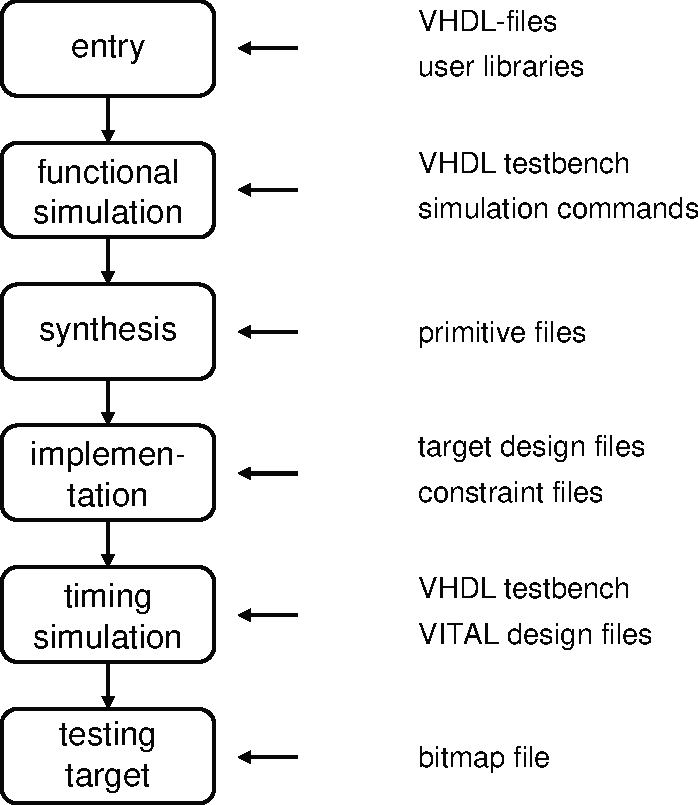
\includegraphics[scale=0.63]{009designflow.pdf}
\caption{De VHDL Design Flow}
\label{fig:009designflow}
\end{figure}

Het bedenken van de schakeling is een creatief proces. Ervaring en goede kennis
van digitale systemen helpt je hierbij op weg. Het opzetten van een goede
simulatie hoort bij de vaardigheden van de ontwerper. De rest wordt eigenlijk
door de tools van Quartus afgehandeld. Het is voor de ontwerper niet meer
interessant om op laag niveau de hardware te bekijken. Je moet er dan
wel zeker van zijn dat je de hardware met de juiste regels beschreven hebt:
combinatoriek en flankgevoelige geheugenelementen. Latches zijn uit den boze.


\chapter{Practicumomgeving}
\label{chap:practicumomgeving}
In dit hoofdstuk wordt de practicumomgeving toegelicht.


\section{Ontwikkelbord}
\label{sec:ontwikkelbord}
Het practicum maakt gebruik van een ontwikkelbordjes, de DE0. Op dit bordje
is een FPGA van Altera geplaatst. Hieronder is een foto weergegeven.

\begin{figure}[H]
\centering
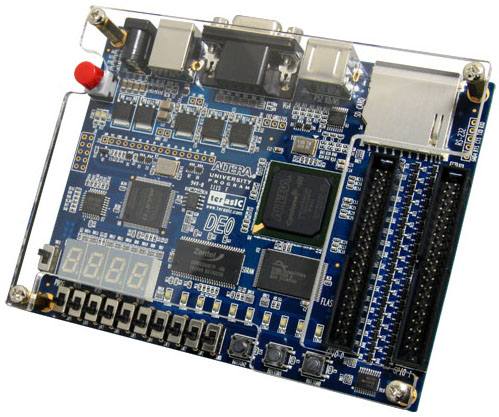
\includegraphics[scale=0.63]{image-de0.jpg}
\caption{Het DE0-ontwikkelbord}
\label{fig:image-de0}
\end{figure}
 
Daarnaast zijn ook nog schakelaars, leds en 7-segment displays aanwezig. Zie
hoofdstuk \ref{chap:ontwikkelbordje} voor meer informatie.

Naast het bordje wordt een softwarepakket van de fabrikant gebruikt genaamd
Quartus II. In de volgende paragraaf wordt een korte beschrijving gegeven van
de software. Je hoeft niet alles in \'{e}\'{e}n keer te kennen. Verderop in
deze handleiding is een tutorial opgenomen die je stap voor stap door het
ontwerptraject loodst.

Om de component te configureren is een (hardware-)programmer nodig. Deze is op
het ontwikkelbord geplaatst. Er is alleen een USB-kabel nodig voor een
verbinding tussen een PC en het ontwikkelbord.

\subsubsection{Quartus II}
Quartus II is een alles-in-\'{e}\'{e}n pakket voor het ontwikkelen van digitale
schakelingen en het configureren van (Altera) componenten. Het bestaat uit een
viertal delen:

\begin{itemize}\itemsep-1pt
\item het invoergedeelte - d.m.v. schema's, VHDL, toestandsdiagrammen
\item synthesizer - dit deel vertaalt de invoer naar een netlist,
\item implemention - genereert een bit-file die je in de component kunt laden,
\item programmer - dit deel configureert de component via de USB-interface.
\end{itemize}

\subsubsection{ModelSim}
ModelSim is een VHDL-simulator die direct vanuit de broncode simuleert. Er zijn
in principe geen tussenstappen nodig zoals synthese. Je kan echter ook de
uitvoer van de synthese simuleren. Hierdoor krijg je inzicht in de
vertragingstijden. Met ModelSim is het mogelijk abstracte beschrijvingen van
digitale schakelingen te simuleren. Deze schakelingen zijn niet
synthetiseerbaar.

ModelSim kan als stand-alone pakket gebruikt worden. Wij zullen ModelSim
gebruiken als onderdeel van Quartus en ModelSim starten vanuit Quartus.


\section{Software-versies en web-edition}
\label{sec:softwareversies}
Het Quartus-pakket komt in twee smaken. Er is een volledige betaalde versie
waarbij een licentie-server nodig is en er is een zogenaamde \textsl{Web
Edition}. De
eerstgenoemde is de meest krachtige versie: alle \textsl{devices} van Altera
zijn hiermee te configureren. Daarnaast heb je hier nog optie-pakketten voor
DSP-ontwikkeling en digitale filters. De Web Wdition is gratis, heeft geen 
licentie-server nodig, maar kan niet synthetiseren voor alle beschikbare IC's.
Er zijn geen optie-pakketten beschikbaar.

Van ModelSim bestaan ook twee versies: de volledige, betaalde Altera-versie en
de zogenaamde \textsl{Altera Starter Edition}. De typering ``Altera'' geeft aan
dat het specifiek ontwikkeld is om met Quartus samen te werken. De betaalde
versie heeft geen beperkingen, de Altera Starter Edition kan maximaal 10000
VHDL-coderegels simuleren en verwerkt de code langzamer dan de betaalde versie.

De Web Edition van Quartus (met ModelSim ge\"{\i}ntegreerd) kan gevonden
worden op

%\hspace*{1cm}\url{https://www.altera.com/download/software/quartus-ii-we}
\hspace*{1cm}\url{http://dl.altera.com/13.0sp1/?edition=web#tabs-1}

%De Starter Edition van ModelSim kan gevonden worden op
%
%\hspace*{1cm}\url{https://www.altera.com/download/software/modelsim-starter}

De software draait op Windows\texttrademark\ \'{e}n Linux\texttrademark\ , er
is geen OS X-versie. Op het practicum wordt Windows gebruikt.

Let erop dat het practicum wordt uitgevoerd met versie 11.1sp1 resp\@. versie
10.0c.

Noot: aangeraden wordt om versie 13.0sp1 te installeren. Hogere versies
ondersteunen de FPGA's (Cyclone II en III) op de gebruikte ontwikkelbordjes
niet. Versie 13.0sp1 is prima geschikt om deze tutorial te doorlopen. Let er
op dat de pictogrammen kunnen afwijken t.o.v.\@ versie 11.1sp1. De in
het practicum gemaakte Quartus-projecten
kunnen zonder problemen door zowel versie 13.0sp1 als 11.1sp1 geopend worden.
Vanaf versie 13.0 is ModelSim ge\"{\i}ntegreerd in het installatiepakket.

%\textbf{
%Let op: versie 14.0 en hoger kunnen niet gebruikt worden i.s.m.\@ het
%DE0-bordje!
%}



\chapter{Ontwikkelbordje}
\label{chap:ontwikkelbordje}
In dit hoofdstuk wordt het ontwikkelbordje nader beschreven. Eerst wordt een
blokschema getoond en worden de diverse onderdelen kort beschreven. Daarna
volgt een paragraaf over de configureerbare component, de Altera Cyclone III,
met specificaties van het gebruikte type.


\section{Blokschema}
\label{sec:blokschema}
Het ontwikkelbord is ontwikkeld door het bedrijf Terasic in samenwerking met
Altera, de fabrikant van de Cyclone III. Een gedetailleerde beschrijving is
niet nodig; we geven slechts een blokschema van de onderdelen. Alles wat je
nodig hebt tijdens het practicum staat hier beschreven. In
figuur~\ref{fig:DE0-layout-yellow-1000} is een foto afgebeeld met de diverse
onderdelen.

%% Moet misschien nog iets groter.
\begin{figure}[H]
\centering
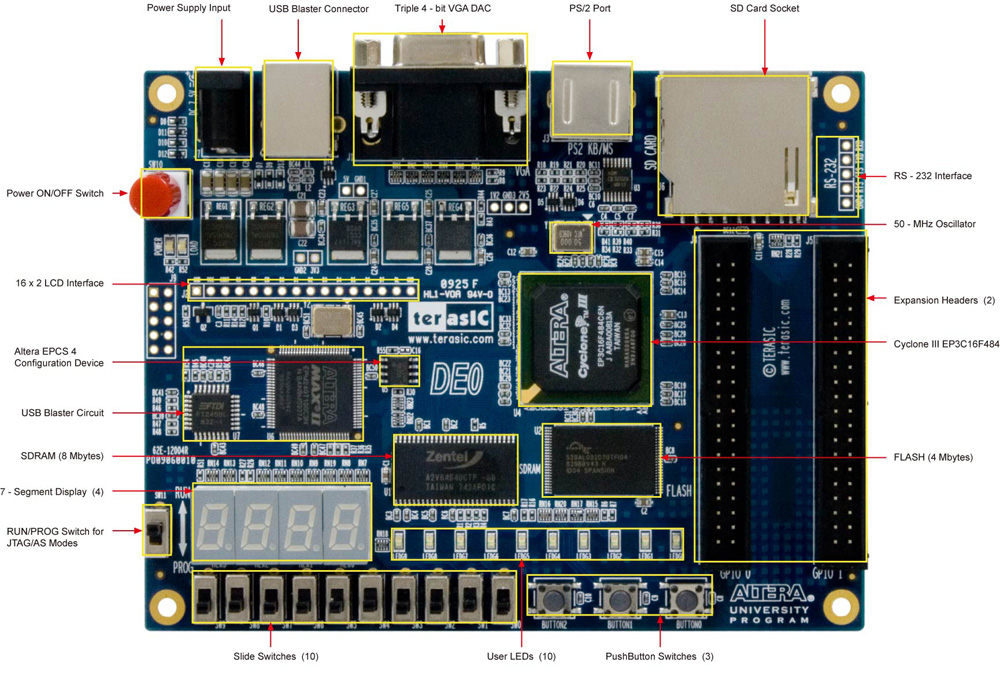
\includegraphics[scale=0.92]{DE0_layout_yellow_1000.jpg}
\caption{Het DE0-ontwikkelbord met benoeming van periferie}
\label{fig:DE0-layout-yellow-1000}
\end{figure}

In figuur~\ref{fig:010blockdiagram} is een blokschema weergegeven. Bij elk
onderdeel staat vermeld met hoeveel signalen het onderdeel verbonden is met de
Cyclone III. De voedingslijnen zijn niet meegenomen. 

\begin{figure}[H]
\centering
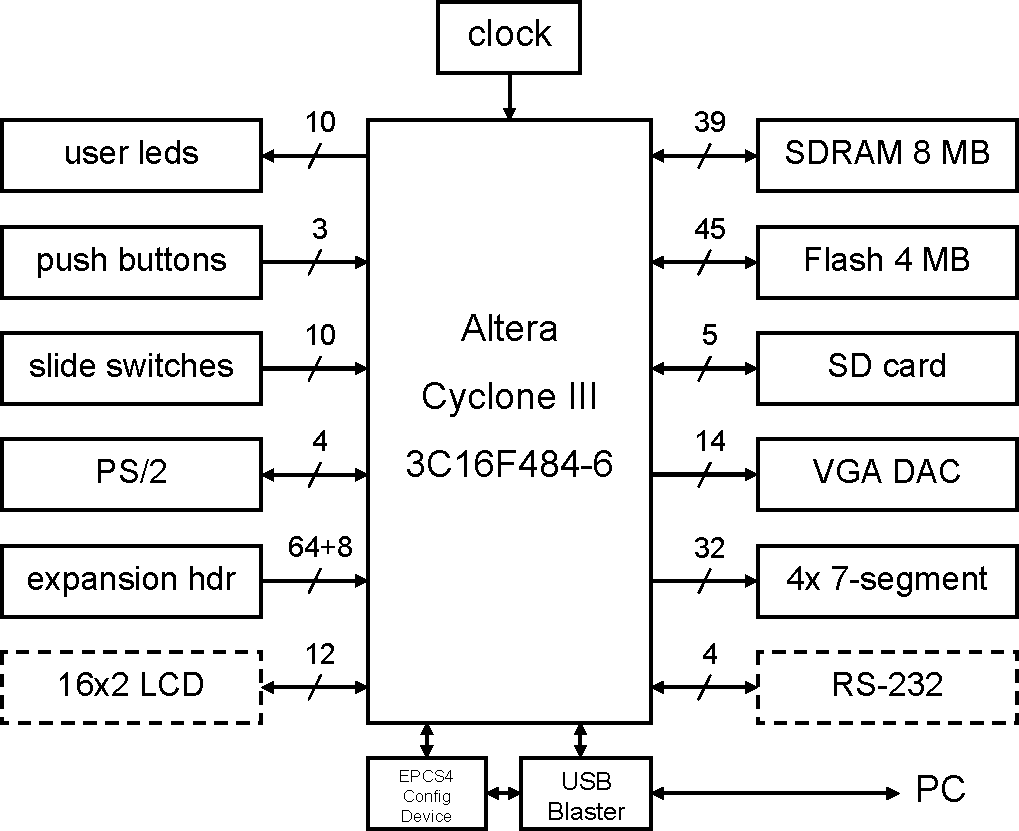
\includegraphics[scale=0.50]{010blockdiagram.pdf}
\caption{Blokschema ontwikkelbord}
\label{fig:010blockdiagram}
\end{figure}

\subsubsection{Cyclone III}
Het hart van het ontwikkelbord wordt gevormd door de Cyclone III EP3C16F484-6N
(zie figuur~\ref{fig:ep3c16f484c6n}). Dit is een configureerbaar IC waarin een
digitale schakeling kan worden geplaatst.

\begin{figure}[H]
\centering
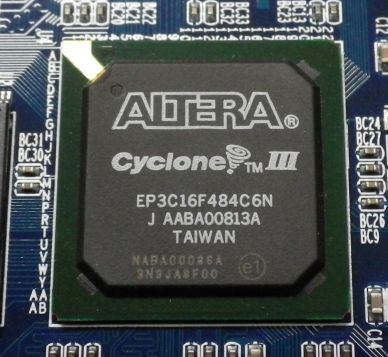
\includegraphics[scale=0.40]{ep3c16f484c6n.jpg}
\caption{Foto Cyclone III}
\label{fig:ep3c16f484c6n}
\end{figure}
%Figuur 3-3  -  foto EP3C16F484C-6N

\subsubsection{Push buttons}
Het ontwikkelbord heeft drie drukknoppen genaamd \naam{BUTTON2} t/m
\naam{BUTTON0}. Deze drukken geven een laag logisch
niveau (0) af als de knop is ingedrukt en een hoog logisch niveau (1) als de
knop niet is ingedrukt. Verder zijn deze drie knoppen ontdenderd en zijn te
gebruiken als kloksignaal.

\subsubsection{Slide switches}
Het ontwikkelbord heeft tien schuifschakelaars genaamd \naam{SW9} t/m
\naam{SW0}. Een schakelaar geeft een laag
logisch niveau (0) af als de schakelaar naar beneden is geschoven (het dichtst
bij de rand van de print) en een hoog logisch niveau (1) als de schakelaar naar
boven is geschoven. Deze schakelaars zijn niet ontdenderd en zijn alleen voor
niveaugevoelige ingangen bedoeld.

\subsubsection{Leds}
Het ontwikkelbord heeft tien groene leds \naam{LEDG9} t/m \naam{LEDG0}. Een
led brandt als een hoog logisch niveau (1) wordt aangeboden en is uit als een
laag logisch niveau (0) wordt aangeboden.

\subsubsection{7-segment displays}
Het ontwikkelbord heeft vier 7-segment displays waarmee getallen van
verschillend formaat kunnen worden gemaakt. Elk display bestaat uit zeven leds
waarmee een cijfer kan worden gevormd. Daarnaast heeft elk display een punt.
Een led brandt als een laag logisch niveau (0) wordt aangeboden en is uit als
een hoog logisch niveau (1) wordt aangeboden.

\subsubsection{Clock}
Het ontwikkelbord heeft \'{e}\'{e}n 50 MHz klokoscillator aan boord. Het
kloksignaal kan dienen als (direct) kloksignaal voor het klokken van flipflops
of als invoer voor een Phase Locked Loop (PLL).

Een overzicht van de pinaansluitingen en de layout van de 7-segment displays
is te vinden in bijlage~\ref{chap:pinbenaming}.

\subsubsection{Overige aansluitingen}
Het ontwikkelbord bevat verder nog een 8 MD SDRAM, een 4 MB Flash, een
VGA-uitgang, een LCD-interface, een SD-card interface, een PS/2-interface, een
RS-232-interface en een expansion header met 64 I/O-lijnen en 8 kloklijnen. Dit
wordt verder niet besproken.


\section{Altera Cyclone III}
\label{sec:alteracycloneiii}
De Cyclone III FPGA (Field Programmable Gate Array)\footnote{Het is wel raar
dat een FPGA configureerbaar heet, terwijl de naam suggereert dat ze
programmeerbaar zijn.} is opgebouwd uit zogenaamde logische elementen (Logic
Elements, LE). Met deze elementen kan je een digitale schakeling bouwen. Het 
gebruikte type heeft er 15408 aan boord. Om een indruk te geven wat dat
inhoudt: een volledige 32-bits processor (NIOS/II) gebruikt zo'n 1800
elementen. Je kan er dus acht processoren in kwijt.

In tabel~\ref{tab:gegevenscyclone} zijn wat gegevens te vinden.
\begin{table}[H]
\caption{Enige gegevens over de EP3C16F484C-6N}
\label{tab:gegevenscyclone}
\centering
\begin{tabular}{|l|l|}
\hline 
Aansluitpinnen (user I/O) & 484 (347) \\ 
\hline 
Logische elementen & 15408 \\ 
\hline 
Geheugenelementen & 15408 (\'{e}\'{e}n per element) \\ 
\hline 
RAM-bits & 516096 \\ 
\hline 
Vermenigvuldigers & 112 (9x9 bit) / 56 (18x18 bit) \\ 
\hline 
Phase Locked Loops & 4 \\ 
\hline 
Global Clock Networks & 20 \\ 
\hline 
$t_{PD(pin-to-pin)}$ & 6 ns \\ 
\hline 
$f_{MAX}$ (I/O, stand alone) & 250 MHz \\ 
\hline 
\end{tabular} 
\end{table}

Figuur~\ref{fig:003chip} geeft een Floor Plan van de bij het practicum gebruikte
3C16. Daarnaast heeft elke Cyclone RAM en vermenigvuldigers aan boord. De
vermenigvuldigers zijn sneller dan wanneer ze met LE's worden opgebouwd.
Je kan ze bijvoorbeeld gebruiken bij digitale signaalbewerking.

\begin{figure}[H]
\centering
%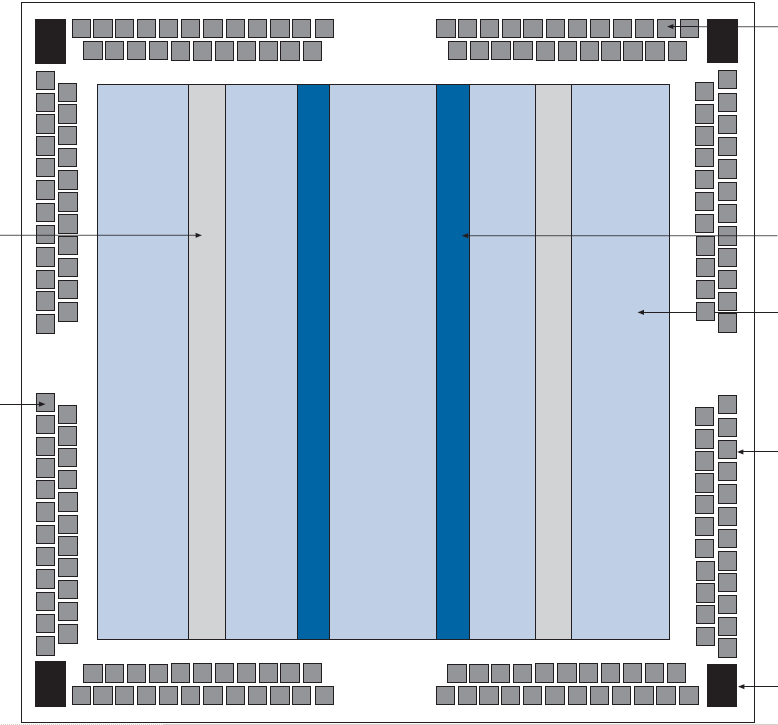
\includegraphics[scale=0.45]{003chip.png}
\begin{overpic}[scale=0.45,unit=1mm]{003chip}
\linethickness{1pt}
\put(-2,51){\makebox(0,0)[r]{\scriptsize 347 user I/O}}
\put(-2,78){\makebox(0,0)[r]{\scriptsize 504 kB embedded memory}}
\put(125,6){\makebox(0,0)[l]{\scriptsize configurable PLL}}
\put(125,43.5){\makebox(0,0)[l]{\scriptsize 250 MHz I/O access}}
\put(125,65.5){\makebox(0,0)[l]{\scriptsize 15048 LE's / 963 LAB's}}
\put(125,77.5){\makebox(0,0)[l]{\scriptsize 112 embedded multipliers}}
\put(125,110.7){\makebox(0,0)[l]{\scriptsize LV-TTL \& CMOS / Tri-state}}
\end{overpic}
\caption{Floor Plan van de Cyclone III}
\label{fig:003chip}
\end{figure}

\subsubsection{Logic Element en Logic Array Block}
Elke LE bestaat uit een 4-input look-up table (LUT) en een D-flipflop. De LE
kan een combinatorische of sequenti\"{e}le functie vervullen. De LUT kan elke
combinatorische schakeling van vier variabelen nabootsen, de D-flipflop kan
\'{e}\'{e}n bit onthouden. Indien je schakeling te groot is om in \'{e}\'{e}n
LE te stoppen wordt dat door de software (synthese, mapper) verdeeld over 
meerdere LE's. Een Logic Array Block bestaat uit 16 LE's en snelle
interconnect.

\subsubsection{Routing en interconnect}
Elke LE kan maar een klein deel van schakeling bevatten. Een schakeling zal dus
uit meerdere LE's bestaan. Tussen de LE's is dus informatie-uitwisseling nodig.
Dat gebeurt door de routing en interconnect. Realiseer je dat zo'n 50\% van het
chipoppervlak alleen maar routing is! De vertragingstijd van combinatorische
schakelingen komt voor 2/3 voor rekening van de routing! Binnen een LAB is
snelle interconnect mogelijk.

\subsubsection{I/O Banks}
De I/O banks (deze chip heeft er acht) zijn verantwoordelijk voor verbindingen
tussen de buitenwereld en het interne gedeelte van de chip. Het levert de
externe signalen netjes af aan de routing en signalen van routing worden netjes
aan de buitenwereld afgeleverd. Tot de mogelijkheden horen: LV-TTL, LV-CMOS
input, tri-state ouput, programmable slew rate.


\chapter{Tutorial met VHDL}
\label{chap:tutorial}
We gaan ons nu bezighouden met het ontwerpen van digitale schakelingen in VHDL.
VHDL is een beschrijvingstaal; het heeft het uiterlijk van een programmeertaal
maar in plaats van machinetaal of binaire code beschrijf je hoe de hardware
moet werken. VHDL leren is een traject apart en komt niet in deze tutorial aan
bod.

Deze tutorial zal je stap voor stap door de diverse onderdelen van Quartus en
Modelsim leiden waarna je zelf een aantal opdrachten moet uitwerken.

De tutorial behandelt slechts een klein gedeelte van alle mogelijkheden die in
Quartus en Modelsim voor handen zijn. Je zal zelf meer functies moeten
onderzoeken die je voor de opdrachten nodig hebt.

We zullen de volgende stappen doorlopen:

\begin{itemize}\itemsep-1pt
\item project aanmaken
\item VHDL code invoeren m.b.v. de HDL editor
\item simuleren van de VHDL code op functioneel niveau 
\item compilatie (synthese en implementatie) van de VHDL code naar een
      configuratiebestand
\item downloaden van de configuratiebestand in de Cyclone III.
\end{itemize}

Niet aan bod komt verificatie. Verificatie valt in twee stukken uiteen: timing
simulatie en timing analyse. De eerste is eigenlijk niets anders dan functionele
simulatie maar dan met inbegrip van timing aspecten. Timing analyse kan je
gebruiken om bijvoorbeeld het langste pad te vinden.

In bijlage~\ref{chap:knoppenensneltoetscombinatie} is een tabel opgenomen met
een aantal knoppen en sneltoetscombinaties. Niet alle knoppen worden in deze
tutorial gebruikt.

\fpf{NB: gebruik geen spaties, leestekens of "vreemde" tekens in mapnamen en
bestandsnamen!}

\section{Quartus starten}
\label{sec:quartusstarten}
Quartus wordt gestart door op het pictogram te klikken of via het Startmenu.
Zie figuur~\ref{fig:020quartus_icon}.

%fig 4-1
\begin{figure}[H]
\centering
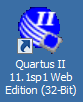
\includegraphics[scale=\tutpicscale]{020quartus_icon.png}
\caption{Quartus II pictogram}
\label{fig:020quartus_icon}
\end{figure}

Na het opstarten \textsl{kan} figuur~\ref{fig:021infoscreen} verschijnen. Via
deze \texttt{Getting Started} kan je snel een project aanmaken of openen. We
slaan dit scherm over. Klik hiervoor op het kruisje rechtsboven.
%fig 4-2
\begin{figure}[H]
\centering
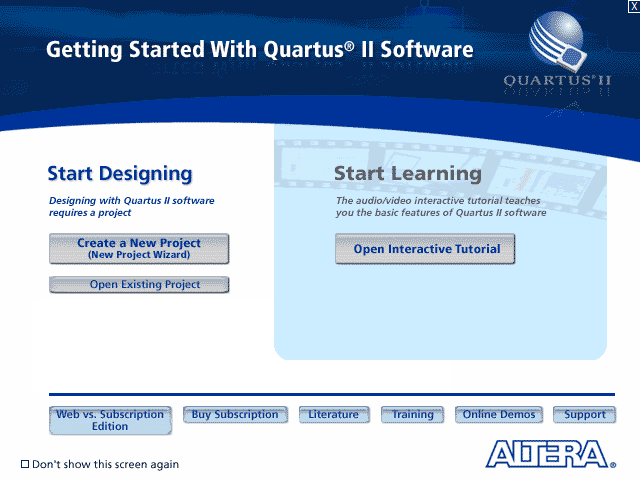
\includegraphics[scale=\tutpicscale]{021infoscreen.png}
\caption{Quartus II opstartscherm}
\label{fig:021infoscreen}
\end{figure}
De Project Manager wordt gestart (figuur~\ref{fig:022projectnavafterstartup}).

%fig 4-3
\begin{figure}[H]
\centering
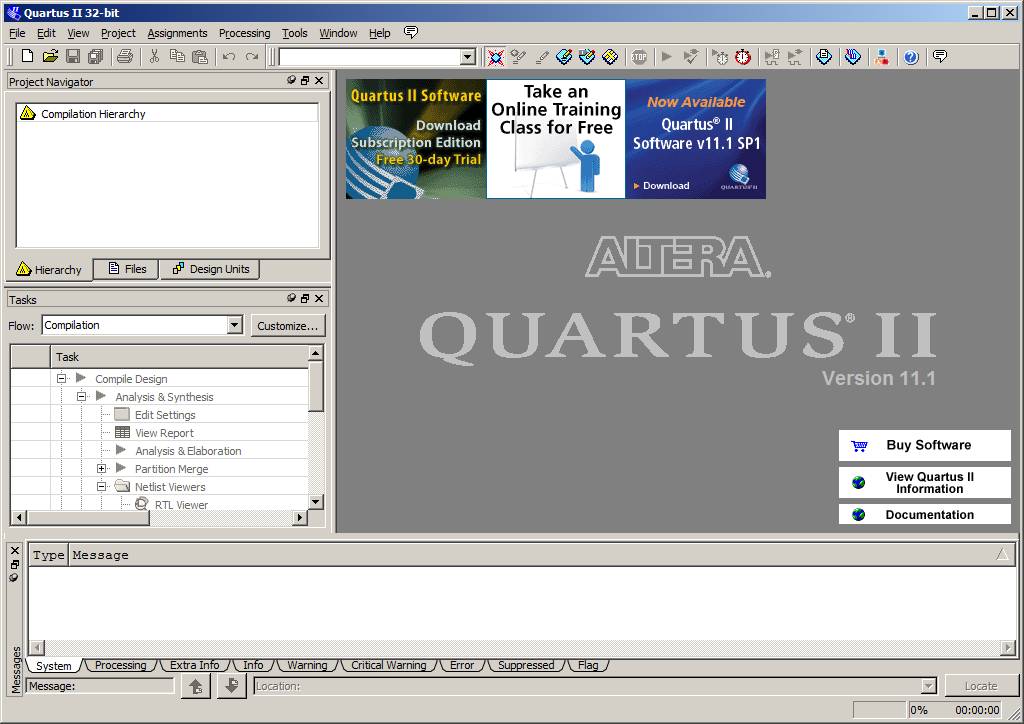
\includegraphics[scale=\tutpicscale]{022projectnavafterstartup.png}
\caption{Openingsscherm project navigator}
\label{fig:022projectnavafterstartup}
\end{figure}

Indien van toepassing, wordt het laatst geopende project geopend.De Project
Manager bestaat uit menu's, knoppenbalk en vier vensters. Linksboven is de
Project Navigator. Hierin worden alle (broncode-)bestanden en de onderlinge 
afhankelijkheden zichtbaar gemaakt, zoals hi\"{e}rarchieen en testbenches.
Daaronder is de Tasks-venster. Hierin worden de mogelijke taken bij een
geselecteerd bestand weergegeven, zoals synthetiseren of implementeren. Rechts
is het edit-venster waar bestanden bewerkt en bekeken kunnen worden. Onderaan
is het Message-venster waar uitvoer van de diverse opdrachten wordt afgedrukt.

\section{Project aanmaken}
\label{sec:projectaanmaken}
Quartus II werkt met zogenaamde projecten als beheerseenheid. In een project
worden alle bestanden ondergebracht die je aanmaakt of die de software
aanmaakt (bijv. output van de synthesizer). Een project is in feite niets
anders dan een map op de harde schijf met daarin alle bijbehorende bestanden.
Voor deze tutorial maken we een nieuw project aan. Klik in de Project Manager
op \menu{File\pijl{}New Project Wizard}.
Zie figuur~\ref{fig:023newprojectwizard}.
 
%fig 4-4
\begin{figure}[H]
\centering
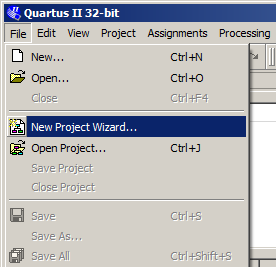
\includegraphics[scale=\tutpicscale]{023newprojectwizard.png}
\caption{Project wizard}
\label{fig:023newprojectwizard}
\end{figure}

Er verschijnt een dialoogscherm zoals in figuur~\ref{fig:024introduction}. Dit
scherm geeft een introductie over de stappen die gaan volgen. Klik op
\menu{Next}.

Nu volgt een nieuw scherm (figuur 4-6). Hierin kan je de projectnaam,
projectmap en projecttype instellen. Zorg ervoor dat je de projecten aanmaakt
op de H-schijf en niet op een USB-stick; Quartus maakt veel bestanden aan en
werken via stick verloopt dan traag.

\fpf{Gebruik geen spaties, leestekens of "vreemde" tekens in mapnamen en
bestandsnamen! \\ Gebruik geen USB-stick. \\ Sla je bestanden op de H-schijf
op.}

Vul de velden in figuur~\ref{fig:025enterdirandname} in zoals is aangegeven.

Let er op dat je de naam in het laatste veld goed invoert. Die naam heb je
nodig bij de entity-beschrijving van je VHDL-beschrijving.
 
%fig 4-5
\begin{figure}[H]
\centering
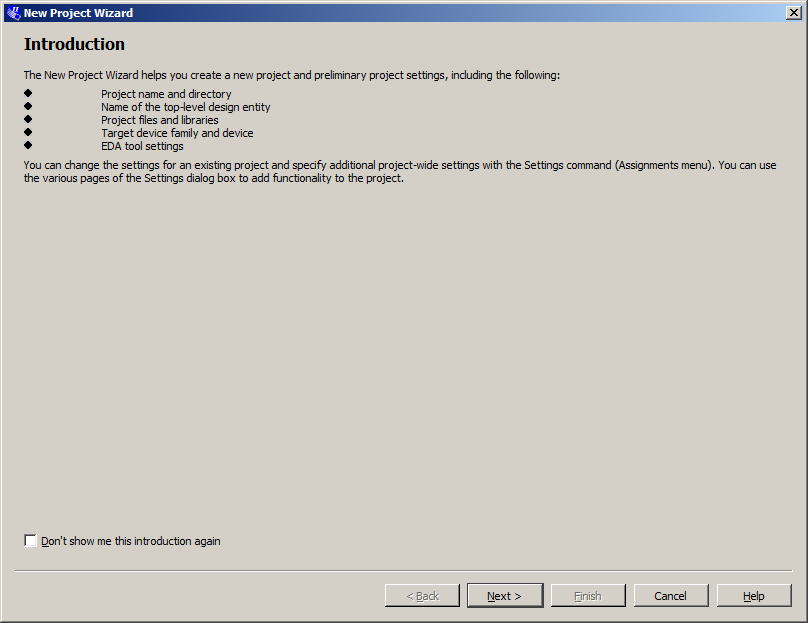
\includegraphics[scale=\tutpicscale]{024introduction.png}
\caption{Introductie project wizard}
\label{fig:024introduction}
\end{figure}

%fig 4-6
\begin{figure}[H]
\centering
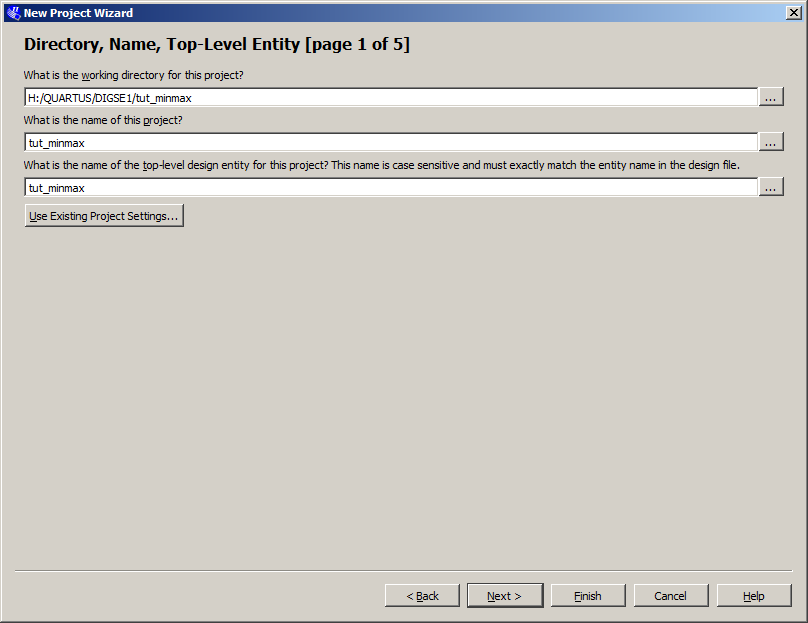
\includegraphics[scale=\tutpicscale]{025enterdirandname.png}
\caption{Invullen mapnaam, projectnaam en naam van de top-level.}
\label{fig:025enterdirandname}
\end{figure}

Na een klik op \menu{Next} wordt nog gemeld dat de opgegeven map niet bestaat
en wordt gevraagd of deze aangemaakt mag worden. Zie
figuur~\ref{fig:026dirdoesnotexist}. 

%fig 4-7
\begin{figure}[H]
\centering
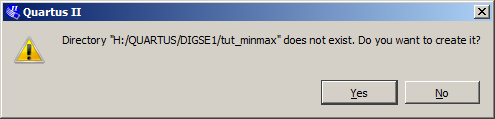
\includegraphics[scale=\tutpicscale]{026dirdoesnotexist.png}
\caption{De map bestaat niet en moet worden aangemaakt.}
\label{fig:026dirdoesnotexist}
\end{figure}

Klik nu op \knop{Yes}. In het volgende scherm kan je bestaande bestanden of
bibliotheken (libraries) opgeven die je in het project wil opnemen
(figuur~\ref{fig:027addfiles}). We maken hier geen gebruik van. Klik op
\knop{Next}.

%fig 4-8
\begin{figure}[H]
\centering
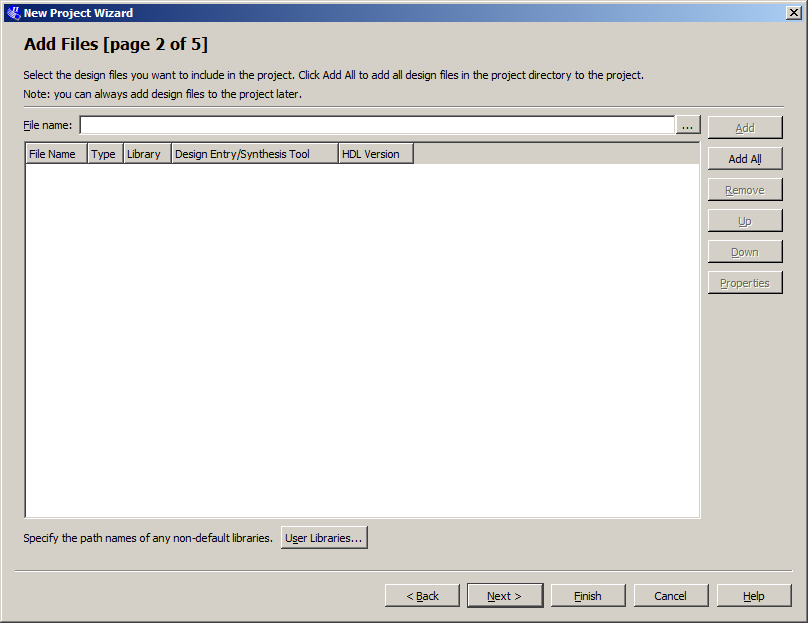
\includegraphics[scale=\tutpicscale]{027addfiles.png}
\caption{Toevoegen van al bestaande bestanden.}
\label{fig:027addfiles}
\end{figure}

Nu wordt een vervolgscherm geopend waarin de device settings worden gevraagd.
Het gebruikte type is een Cyclone III, FBGA (Fine Ball Grid Array) met 484
pinnen en Speed Grade 6. Vul eerst de velden in bij \naam{Device Family},
\naam{Target Device} en \naam{Show in 'Available devices' list} zoals
aangegeven in figuur~\ref{fig:028familydevicesettings}. Daarna selecteer je in
het veld \naam{Available Devices} het type EP3C16F484C6, de eerste uit de
lijst. Klik daarna op \knop{Next}.

In het volgende scherm (figuur~\ref{fig:029edatoolsettings}) kies je als
simulatie-tool ModelSim-Altera met VHDL als taal. Zorg dat het vinkje bij
\naam{Run gate level simulation automaticly after compilation} uit staat.
Klik daarna op \knop{Next}.
 
%fig 4-9
\begin{figure}[H]
\centering
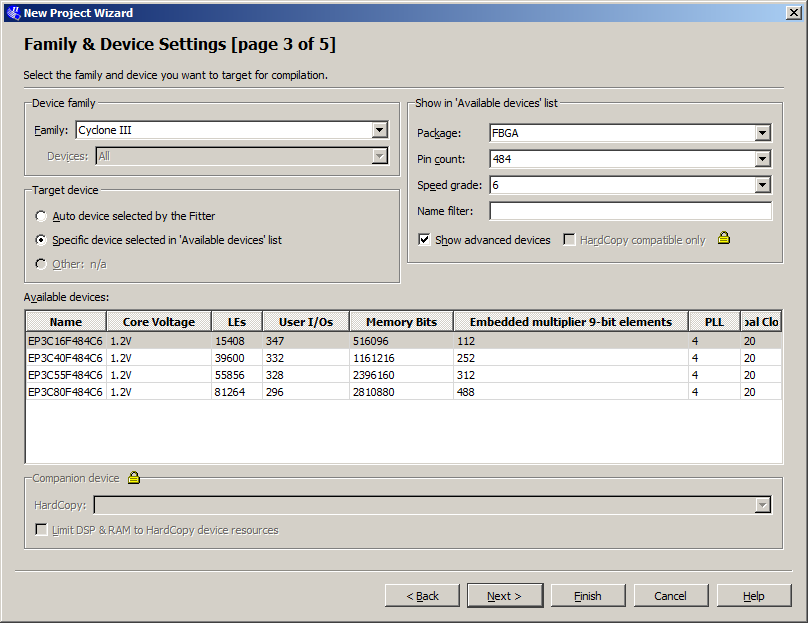
\includegraphics[scale=\tutpicscale]{028familydevicesettings.png}
\caption{Invoeren van device-gegevens.}
\label{fig:028familydevicesettings}
\end{figure}
 
%fig 4-10
\begin{figure}[H]
\centering
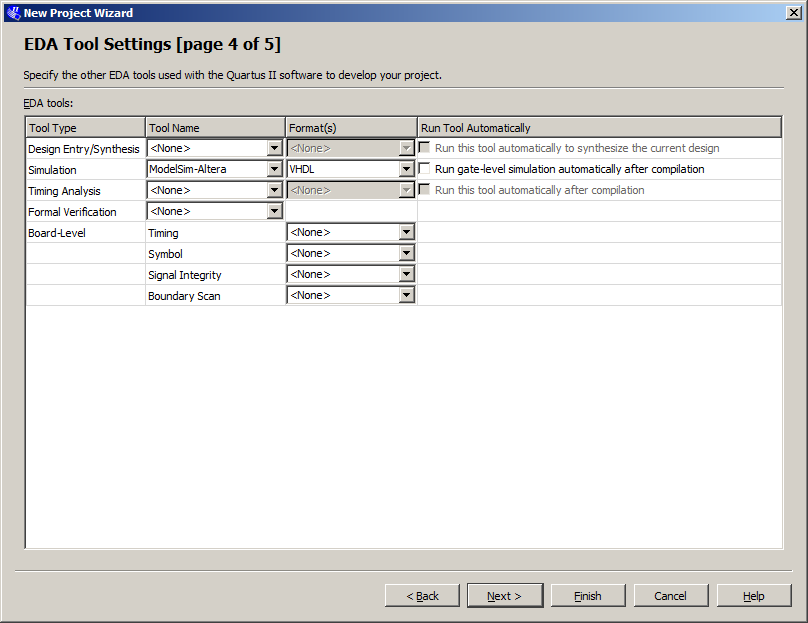
\includegraphics[scale=\tutpicscale]{029edatoolsettings.png}
\caption{Invoeren van EDA tools.}
\label{fig:029edatoolsettings}
\end{figure}

Het laatste scherm van de Project Wizard geeft een overzicht van de gemaakte
keuzen. Zie figuur~\ref{fig:030summary}. Als er iets niet klopt kan je nog
terug. Veel keuzen zijn in een later stadium nog aan te passen. Klik op
\knop{Finish} om de wizard af te sluiten.

%fig 4-11
\begin{figure}[H]
\centering
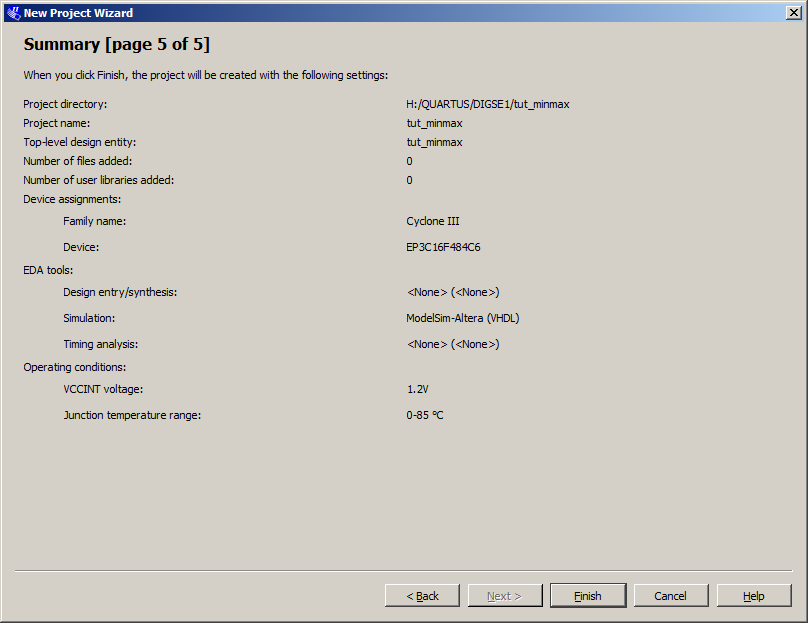
\includegraphics[scale=\tutpicscale]{030summary.png}
\caption{Opsomming van gemaakte keuzen in de project wizard.}
\label{fig:030summary}
\end{figure}

In de titelbalk van de Project Manager verschijnt de naam van project. In de
Project Navigator linksboven verschijnt de gebruikte Altera-component en
daaronder het top-level design name. Zie
figuur~\ref{fig:032projectnavigator_exerpt}.

Opmerking: je kan later de top-level design name nog veranderen. Zie
paragraaf \ref{sec:fouttoplevel}.
 
%fig 4-12
\begin{figure}[H]
\centering
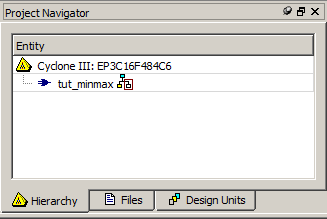
\includegraphics[scale=\tutpicscale]{032projectnavigator_exerpt.png}
\caption{De top-level naam verschijnt in de Project Navigator.}
\label{fig:032projectnavigator_exerpt}
\end{figure}


\section{Invoeren van VHDL-broncode}
\label{sec:invoerenvhdlbroncode}
Als eerste zullen we een VHDL-bestand in het project aanmaken. Klik in de
Project Manager op \menu{File\pijl{}New} (figuur~\ref{fig:040createnewfile}).
 
%fig 4-13
\begin{figure}[H]
\centering
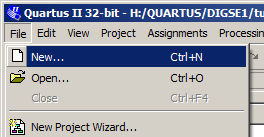
\includegraphics[scale=\tutpicscale]{040createnewfile.png}
\caption{Aanmaken nieuw bestand.}
\label{fig:040createnewfile}
\end{figure}

Nu verschijnt er een scherm waarin je het type van het nieuwe bestand kan
kiezen (figuur~\ref{fig:041newfiledialog}). Kies voor \naam{VHDL file}.
 
%fig 4-14
\begin{figure}[H]
\centering
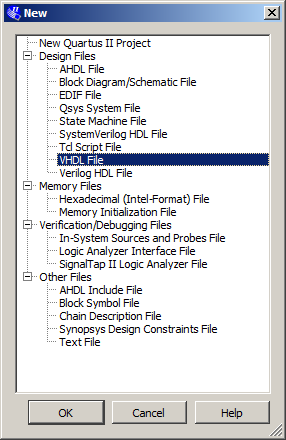
\includegraphics[scale=\tutpicscale]{041newfiledialog.png}
\caption{Keuze bestandstype.}
\label{fig:041newfiledialog}
\end{figure}

De Project Manager opent nu een leeg bestand. Dit is te zien in
figuur~\ref{fig:042projectmanagerwithemptyfile}. Merk op dat het bestand de
tijdelijk naam \naam{Vhd1.vhd} heeft. Bij het opslaan van het bestand kan
alsnog een andere naam worden ingevoerd.

Voer nu de code in zoals is weergegeven in figuur~\ref{fig:044onlythecode}. De
VHDL-code in het edit-venster wordt overzichtelijk gehouden door het gebruik
van kleuren. Groen is voor commentaar, blauw is voor zogenaamde keywords, roze
is voor alles wat met het type \naam{std\_logic} te maken heeft, rood is voor
getallen en zwart is voor de overige tekens en woorden.

Merk op dat de entity de naam \naam{tut\_minmax} heeft. Deze is eerder
opgegeven als zogenaamde top level design entity (zie
figuur~\ref{fig:025enterdirandname}).

Heb je enig idee wat de werking is van deze in VHDL beschreven hardware? Dat
maakt het doorlopen van deze tutorial nog leuker.

%fig 4-15
\begin{figure}[H]
\centering
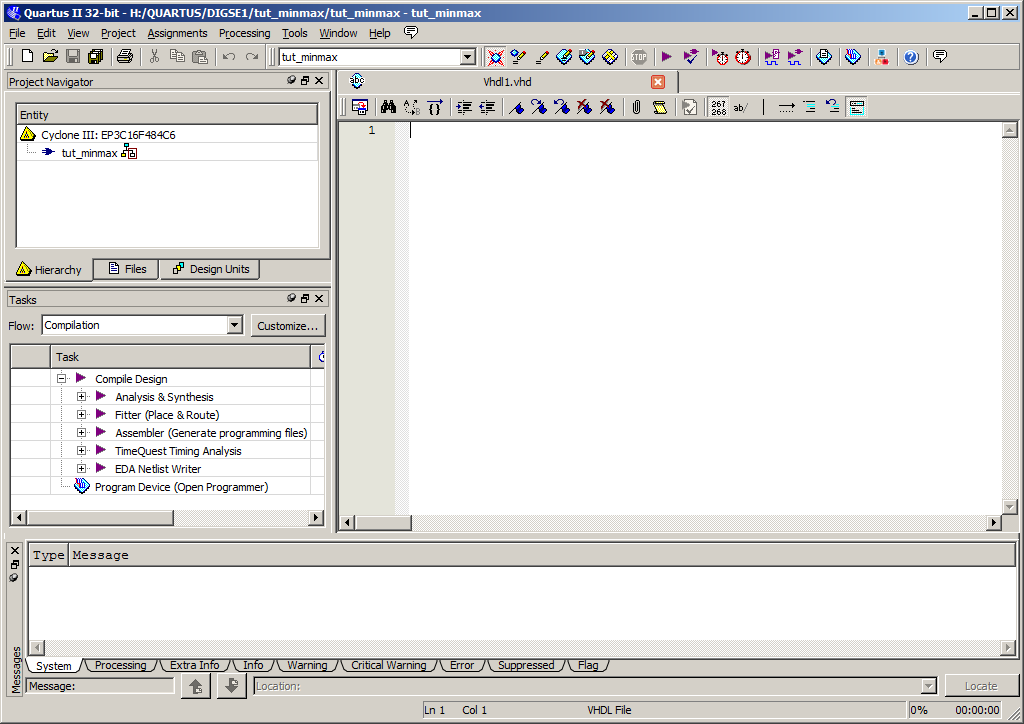
\includegraphics[scale=\tutpicscale]{042projectmanagerwithemptyfile.png}
\caption{Overzicht Quartus IDE na aanmaken nieuw VHDL-bestand.}
\label{fig:042projectmanagerwithemptyfile}
\end{figure}
 
%fig 4-16
\begin{figure}[H]
\centering
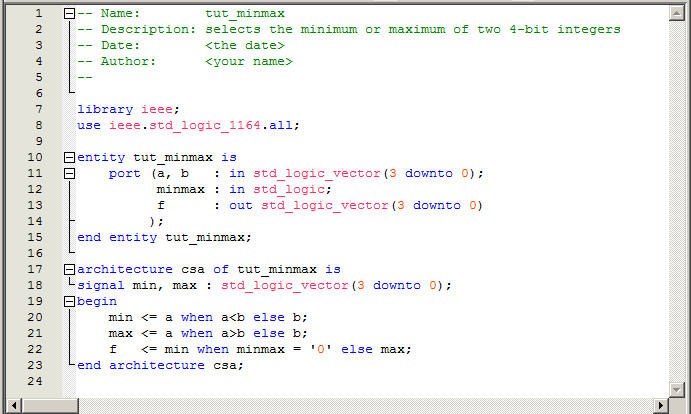
\includegraphics[scale=\tutpicscale]{044onlythecode.png}
\caption{Screenshot van de in te voeren VHDL-code.}
\label{fig:044onlythecode}
\end{figure}

Nu de code is ingevoerd, moet het bestand opgeslagen worden. Klik in de
Project Manager op \menu{File\pijl{}Save} (zie figuur~\ref{fig:045savefile}).
 
%fig 4-17
\begin{figure}[H]
\centering
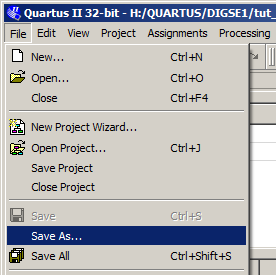
\includegraphics[scale=\tutpicscale]{045savefile.png}
\caption{Opslaan VHDL-bestand.}
\label{fig:045savefile}
\end{figure}

Er wordt een scherm geopend waarin de juiste map en de bestandsnaam ingevuld
kunnen worden. Zie figuur~\ref{fig:046savefiledialog}. Er wordt een
bestandsnaam voorgesteld, dit kan je wijzigen. Let op het vinkje bij
\naam{Add file to current project}.
 
%fig 4-18
\begin{figure}[H]
\centering
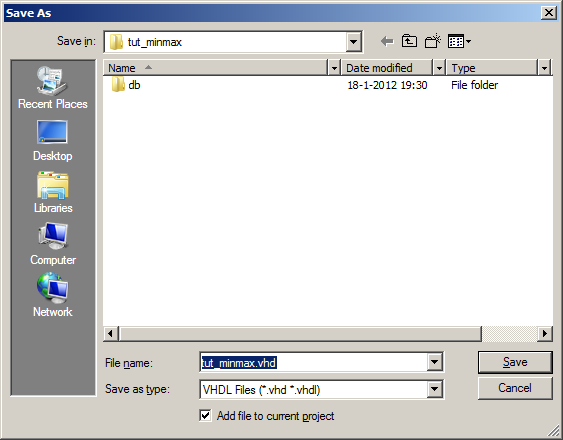
\includegraphics[scale=\tutpicscale]{046savefiledialog.png}
\caption{Opgeven bestandsnaam VHDL-bestand.}
\label{fig:046savefiledialog}
\end{figure}

\textbf{Noot:} je mag geen spaties, leestekens of "vreemde" tekens in de
bestandsnaam opnemen! \\
\textbf{Noot:} let goed op de map waarin het bestand opgeslagen wordt. Quartus
wil nog wel eens de map van een eerder geopend project presenteren.

Het bestand is nu terug te vinden in de Project Navigator onder het tabblad
\naam{Files}. Zie figuur~\ref{fig:047fileinfilestab}.
 
%fig 4-19
\begin{figure}[H]
\centering
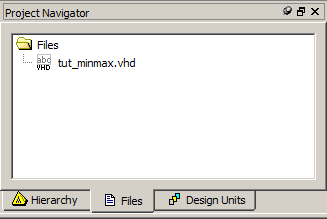
\includegraphics[scale=\tutpicscale]{047fileinfilestab.png}
\caption{Het opgeslagen bestand staat in de lijst van bestanden.}
\label{fig:047fileinfilestab}
\end{figure}

Om te controleren of de VHDL-code syntactisch correct is en er hardware voor
kan worden gegenereerd zullen we de synthesizer starten. Klik in de Project
Manager op \menu{Processing\pijl{}Start\pijl{}Start Analysis \& Synthesis} of
gebruik de sneltoetscombinatie \menu{Ctrl+K}. Zie
figuur~\ref{fig:080startanalysisandsynthesis}.
 
%fig 4-20
\begin{figure}[H]
\centering
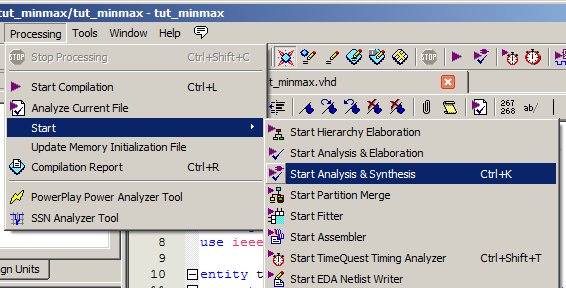
\includegraphics[scale=\tutpicscale]{080startanalysisandsynthesis.png}
\caption{Starten Analysis \& Synthesis vanuit het menu.}
\label{fig:080startanalysisandsynthesis}
\end{figure}

Als deze stap gelukt is zie je onder \naam{Tasks} een paar vinkjes verschijnen
en je krijgt een melding (figuur~\ref{fig:081succesfull}). Klik op \knop{OK} om
verder te gaan.
 
%fig 4-21
\begin{figure}[H]
\centering
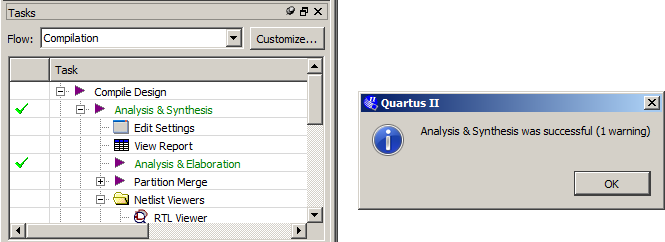
\includegraphics[scale=\tutpicscale]{081succesfull.png}
\caption{De analyse is gelukt.}
\label{fig:081succesfull}
\end{figure}

Mocht je een fout hebben gemaakt, bijvoorbeeld het vergeten van een punt-komma,
dan zal de analyser dat melden, zie figuur~\ref{fig:075notsuccessfull}.

%fig 4-22
\begin{figure}[H]
\centering
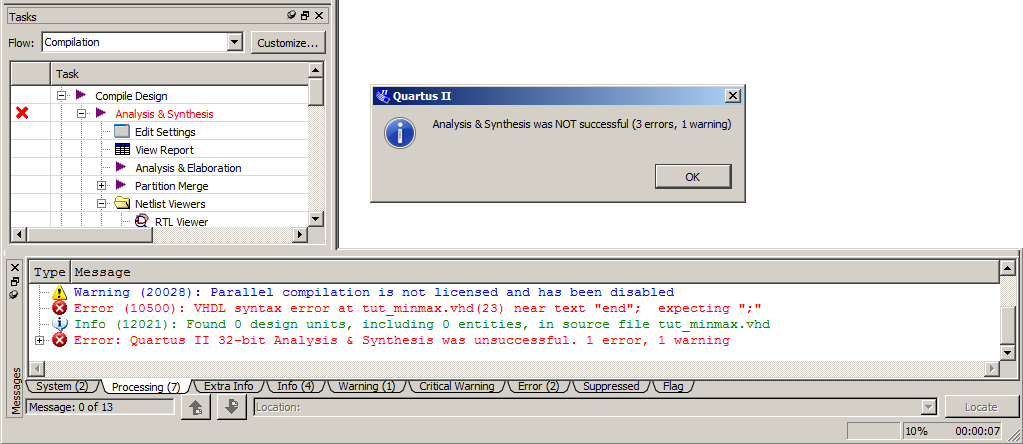
\includegraphics[scale=\tutpicscale]{075notsuccessfull.png}
\caption{De analyse is mislukt.}
\label{fig:075notsuccessfull}
\end{figure}

\section{Simulatie VHDL-broncode}
\label{sec:simulatievhdlbroncode}
Nu de code geschreven is, dient het gesimuleerd te worden. Dit droogzwemmen is
bedoeld om te kunnen verifi\"{e}ren of de schakeling, en dus de VHDL-code,
werkt volgens de specificaties. Het Quartus II pakket gebruikt hiervoor de
externe simulator ModelSim van firma ModelTech. We gebruiken de simulator om
aan te tonen dat onze VHDL-code functioneel correct is. Het kan namelijk best
zijn dat de VHDL-code gesynthetiseerd kan worden, maar dat de schakeling niet 
doet wat het moet doen. Bij deze simulatie worden geen vertragingstijden
meegenomen.

Voor simulatie zijn twee bestanden nodig: een testbench en een commandobestand.
Een testbench is een VHDL-bestand met daarin stimuli dat voor simulatiedoeleinden
is geschreven. Je beschrijft hier de waarden van de ingangen (ports) in de tijd
gezien. Het is een sequentie van toekenning. Het tweede bestand is een
zogenaamd commandobestand: hierin staan opdrachten voor de simulator. De
commando's zijn onderdeel van de script-taal Tcl (``Tickle''). Je kan
deze opdrachten ook interactief op een commandoregel invoeren, maar vaak wil
je de simulatie een paar keer opnieuw draaien. Dan is het steeds invoeren van
de (zelfde reeks) commando's een tijdrovende zaak.

Noot: de hier beschreven wijze van simuleren wijkt een klein beetje af van de
gebruikelijke methode zoals dit normaal in Quartus wordt gedaan. Verderop in de
tutorial wordt hier nog wat meer over beschreven.

De testbench begint met een \texttt{wait}-statement van 10 ns (nanoseconden;
simulatietijd, geen echte tijd). Merk op dat eerst gewacht wordt; de ingangen
van de VHDL-beschrijving zijn dan nog niet gedefinieerd. Dat is straks ook
terug te zien in de simulatieresultaten. Na 10 ns wordt ingang \texttt{A} op
1011$_2$ (11$_{10}$) gezet (merk op dat dit vier bits zijn) en ingang
\texttt{B} op 1001$_{2}$ (9$_{10}$) gezet. Ingang \texttt{minmax} wordt op 0
gezet. Er wordt weer 10 ns gewacht. Zo worden alle combinaties met \texttt{A},
\texttt{B} en \texttt{minmax} gesimuleerd. De laatste wachtopdracht zorgt
ervoor dat de simulator zal stoppen.

Maak een nieuw broncodebestand aan via het menu \menu{File\pijl{}New} en kies
\naam{VHDL File} (zie de figuren~\ref{fig:040createnewfile} en
\ref{fig:041newfiledialog}).Er wordt nu een leeg scherm geopend. Vul hier de
testbenchcode uit listing~\ref{cod:vhdltestbench} op
pagina~\pageref{cod:vhdltestbench} in. Geef het bestand de naam
\naam{tb\_tut\_minmax.vhd} en sla het op. Zie figuur~\ref{fig:062savefile}.

\begin{lstlisting}[language=VHDL,caption=VHDL-testbench,label=cod:vhdltestbench,float=p,numbers=none]
-- Name:        tb_tut_minmax
-- Description: testbench for tut_minmax
-- Date:        <the date>
-- Author:      <your name>
--

library ieee;
use ieee.std_logic_1164.all;

-- Empty entity
entity tb_tut_minmax is
end tb_tut_minmax;

architecture sim of tb_tut_minmax is
-- Top level signals
signal a, b   : std_logic_vector(3 downto 0);
signal minmax : std_logic;
signal f      : std_logic_vector(3 downto 0);

-- Component declaration
component tut_minmax is
   port (a, b    : in std_logic_vector(3 downto 0);
         minmax  : in std_logic;
         f       : out std_logic_vector(3 downto 0)
        );
end component tut_minmax;

begin
   -- Component instantiation
   dut : tut_minmax 
         port map (a => a, b => b, minmax => minmax, f => f);

   -- Process that asserts the stimuli
   stim: process is
   begin
      wait for 10 ns;
      a <= "1011"; b <= "1001"; minmax <= '0';
      wait for 10 ns;
      minmax <= '1';
      wait for 10 ns;
      a <= "0011"; b <= "1100"; minmax <= '0';
      wait for 10 ns;
      minmax <= '1';
      wait;   -- wait forever
   end process;
	
end sim;
\end{lstlisting}

%fig 4-23
\begin{figure}[H]
\centering
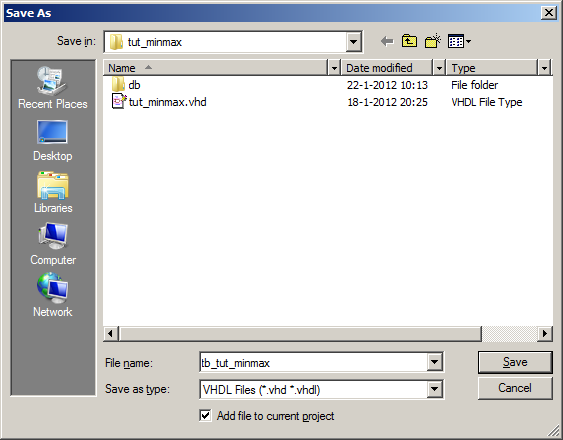
\includegraphics[scale=\tutpicscale]{062savefile.png}
\caption{Aanmaken VHDL-testbench-bestand.}
\label{fig:062savefile}
\end{figure}
 
Het bestand wordt nu echter gezien als een VHDL-broncodebestand en niet als
een testbench. Hiervoor moeten we het type wijzigen. Klik in de Project
navigator met de \textbf{rechter} muisknop op de naam
\naam{tb\_tut\_minmax.vhd} om een menu te openen. Selecteer \menu{Properties}
in het menu (figuur~\ref{fig:063changeproperties}).
 
%fig 4-24
\begin{figure}[H]
\centering
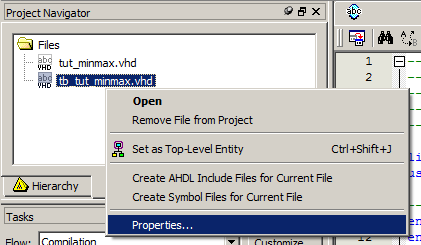
\includegraphics[scale=\tutpicscale]{063changeproperties.png}
\caption{Aanpassen bestandseigenschappen.}
\label{fig:063changeproperties}
\end{figure}

Selecteer in het veld \naam{Type:} de optie \naam{VHDL Test Bench File}. Klik dan op \menu{Ok}
(figuur~\ref{fig:064changedtotestbench}).
 
%fig 4-25
\begin{figure}[H]
\centering
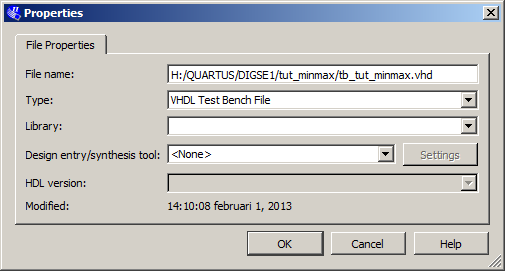
\includegraphics[scale=\tutpicscale]{064changedtotestbench.png}
\caption{Bestandstype veranderd naar VHDL-testbench.}
\label{fig:064changedtotestbench}
\end{figure}

In de Project Navigator is nu zichtbaar dat het type is veranderd (figuur~\ref{fig:065projectnavfiletypechanged}).
 
%fig 4-26
\begin{figure}[H]
\centering
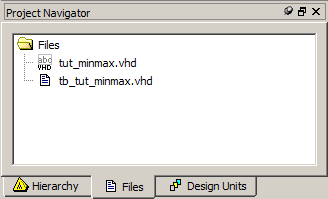
\includegraphics[scale=\tutpicscale]{065projectnavfiletypechanged.png}
\caption{Overzicht bestanden en bestandstypen.}
\label{fig:065projectnavfiletypechanged}
\end{figure}

De volgende stap is het aanmaken van het commandobestand. Klik in de Project
Manager op menu \menu{File\pijl{}New} en kies \naam{Text File} (zie de
figuren~\ref{fig:040createnewfile} en \ref{fig:066newfiledialogbox}). Er wordt
nu een leeg scherm geopend.

%fig 4-27
\begin{figure}[H]
\centering
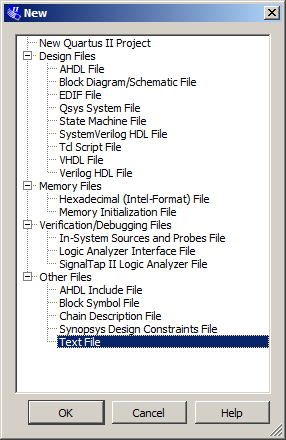
\includegraphics[scale=\tutpicscale]{066newfiledialogbox.png}
\caption{Aanmaken ModelSim commando-script.}
\label{fig:066newfiledialogbox}
\end{figure}

Vul de code in zoals is weergegeven in listing~\ref{cod:modelsimscript} op
pagina~\pageref{cod:modelsimscript}.

Noot: in de code zijn twee padnamen opgenomen die beginnen met punten (\naam{../../}). Dit is een 
verwijzing naar twee hoger gelegen mappen. Quartus plaatst allerlei bestanden in de map genaamd
\naam{simulation/modelsim} die onder de project-map geplaatst is en start de simulatie vanaf dat 
punt. Wij hebben echter onze testbench en commandobestand in project-map geplaatst. Vandaar 
dat bij de compileeropdrachten dus een dubbele verwijzing naar een hoger gelegen padnaam 
moet worden gebruikt.

\begin{lstlisting}[language=tclfix,caption=ModelSim command script,label=cod:modelsimscript,float=p,numbers=none]
# Name:        tb_tut_minmax.do
# Description: script for running simulation
# Date:        <the date>
# Author:      <your name>

# Set transcript on
transcript on

# Recreate the work directory and map to work
if {[file exists rtl_work]} {
    vdel -lib rtl_work -all
}
vlib rtl_work
vmap work rtl_work

# Compile the Tutorial description and testbench. Note the double
# parent references in the path name
vcom -93 -work work ../../tut_minmax.vhd
vcom -93 -work work ../../tb_tut_minmax.vhd

# Start the simulator with 1 ns time resolution
vsim -t 1ns -L rtl_work -L work -voptargs="+acc" tb_tut_minmax

# Log all signals in the design, good if the number of signals is small.
add log -r *

# Add all toplevel and simulated device signals to the list view
add list *
add list dut/*

# Add all toplevel signals and a number of signals inside
# the simulated design to the wave view
add wave -divider "Inputs"
add wave a
add wave b
add wave minmax
add wave -divider "Internals"
add wave dut/min
add wave dut/max
add wave -divider "Outputs"
add wave f

# Open the List and Waveform window
view list
view wave

# Run simulation for 50 ns
run 50 ns

# Fill up the waveform in the window
wave zoom full
\end{lstlisting}

Sla het bestand op, maar let op! De extensie moet in \naam{.do} veranderd worden!
Zie figuur~\ref{fig:067saveasdofile}.

%fig 4-28
\begin{figure}[H]
\centering
%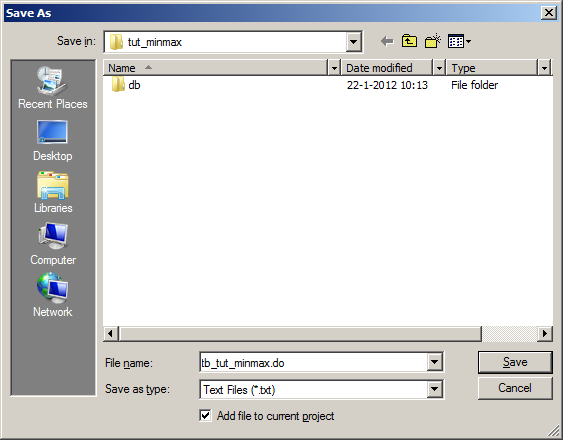
\includegraphics[scale=\tutpicscale]{067saveasdofile.png}
\begin{overpic}[scale=\tutpicscale,unit=1mm]{067saveasdofile.png}
\linethickness{1pt}
\color{red}\put(48.5,12.25){\oval(45,5)}
\end{overpic}
\caption{Naamgeving ModelSim commando-script aanmaken.}
\label{fig:067saveasdofile}
\end{figure} 

Nu moeten we de simulatie-omgeving instellen. Selecteer via het menu 
\menu{Assignments\pijl{}Settings} of gebruik de sneltoetscombinatie
\menu{Ctrl+Shift+E}. Zie figuur~\ref{fig:074assignmentssettings}.

%fig 4-29
\begin{figure}[H]
\centering
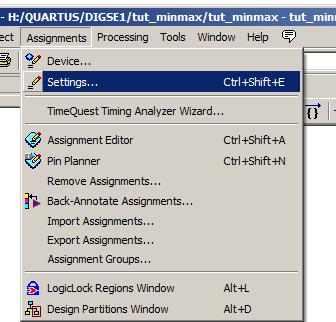
\includegraphics[scale=\tutpicscale]{074assignmentssettings.png}
\caption{Project settings aanpassen.}
\label{fig:074assignmentssettings}
\end{figure} 

Er wordt nu een nieuw scherm geopend waarin de instellingen van het project
gewijzigd kunnen worden. Selecteer in het gedeelte \naam{Catagory} de optie
\naam{EDA Tool Settings - Simulation} (zie
figuur~\ref{fig:073settingssimulation}). Aan de rechterkant verschijnen de
instellingen voor de simulatie. De toolnaam moet op \naam{ModelSim-Altera}
staan de optie \menu{Run gate-level simulation} moet uit staat.

Vink onder \naam{NativeLink Settings} de optie \naam{Script to compile
testbench} aan. In het bijbehorende veld moet je de naam van het commandobestand
invullen. Je kunt ook het bestand selecteren door op de knop met de drie
puntjes te klikken. Er wordt dan een venster geopend waarin je een bestand kan
selecteren (geen figuur).

%fig 4-30
\begin{figure}[H]
\centering
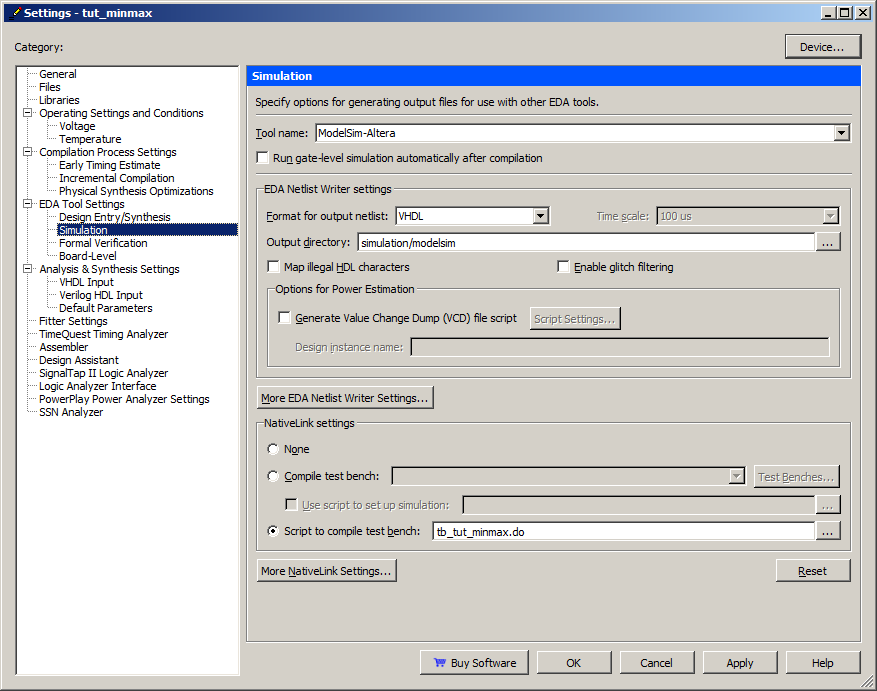
\includegraphics[scale=\tutpicscale]{073settingssimulation.png}
\caption{Invoeren settings voor simulatie met ModelSim}
\label{fig:073settingssimulation}
\end{figure} 

Klik daarna op \menu{Apply} en \menu{OK}. Het scherm wordt afgesloten.

Nu moet de simulatie gestart worden. Klik in de Project Manager op de menu-optie 
\menu{Tools\pijl{}Run Simulation Tool\pijl{}RTL Simulation}. De simulator wordt gestart via 
Quartus. 

Noot: voordat de simulator gestart kan worden, moet de beschrijving geanalyseerd en 
gesynthetiseerd zijn. Zie de figuren~\ref{fig:080startanalysisandsynthesis} tot en met
\ref{fig:075notsuccessfull}. Als dat niet gebeurt is krijg je de volgende 
foutmelding (figuur~\ref{fig:077nativelinkneedssynthesis}).

%fig 4-31
\begin{figure}[H]
\centering
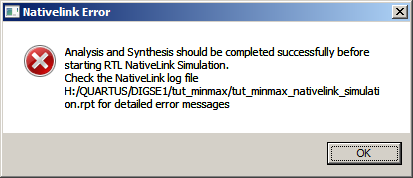
\includegraphics[scale=\tutpicscale]{077nativelinkneedssynthesis.png}
\caption{Foutmelding dat synthese nog niet gelukt is.}
\label{fig:077nativelinkneedssynthesis}
\end{figure} 

Noot: voordat de simulator gestart kan worden, moet je eerst het pad naar de simulator instellen, 
anders volgt een foutmelding. Zie paragraaf~\ref{chap:instellenmodelsimpad}.

Tijdens het starten van Modelsim wordt een \textsl{splashscreen} getoond. De simulator wordt gestart 
(dit kost enige tijd) en er worden vijf vensters geopend (zie figuur~\ref{fig:071modelsimaftersimulationready}).

%fig 4-32
\begin{figure}[H]
\centering
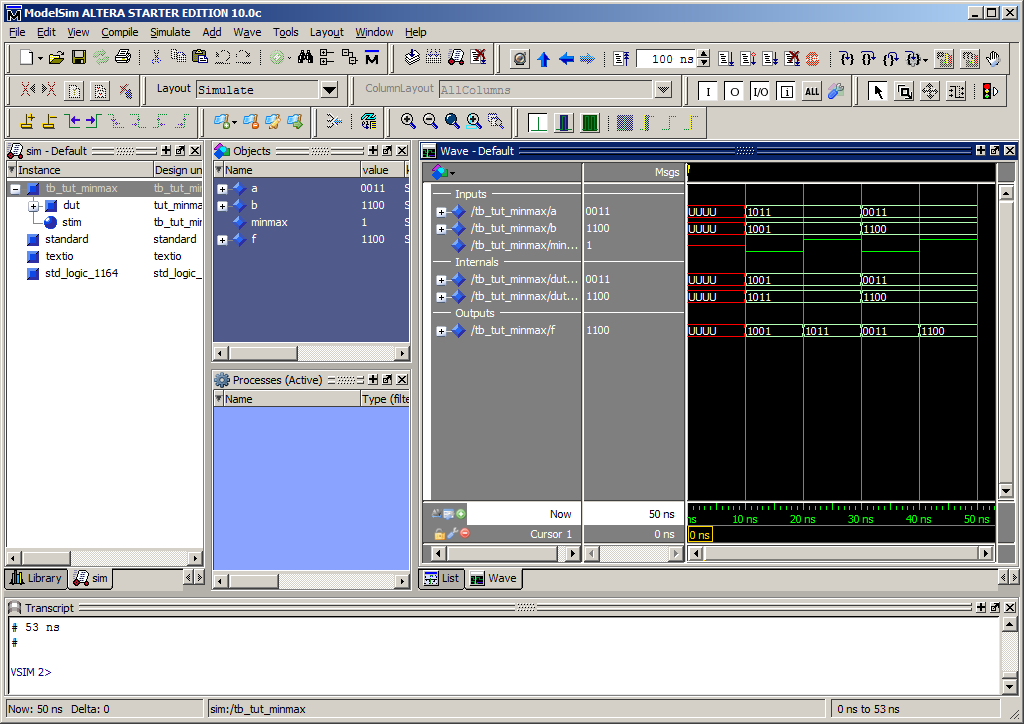
\includegraphics[scale=\tutpicscale]{071modelsimaftersimulationready.png}
\caption{Overzicht ModelSim IDE na het uitvoeren van het commando-script.}
\label{fig:071modelsimaftersimulationready}
\end{figure}
 
Onderaan is het \textsl{Transcript Window}. Hier kan je ook losse commando's geven
(voor gevorderen). Rechts is het \textsl{Waveform Window}.
De overige drie zijn niet nu niet van belang.

In figuur~\ref{fig:072viewwindowonlywithmarkers} is de \textsl{Waveform Window}
te zien. Hierin wordt een tijddiagram afgebeeld van de 
simulatie. Het beste kan je dit venster maximaliseren, zeker als er veel signalen zijn en er voor 
langere tijd gesimuleerd wordt.

%fig 4-33
\begin{figure}[H]
\centering
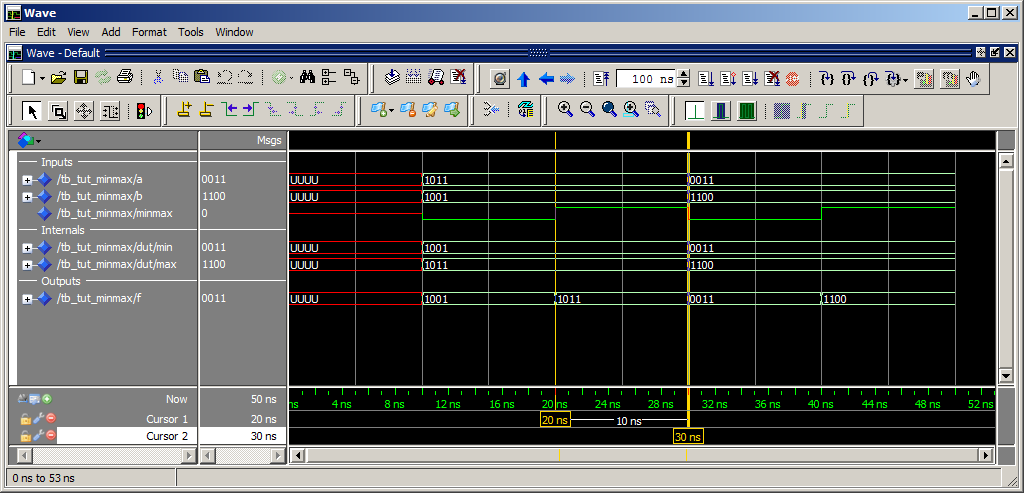
\includegraphics[scale=\tutpicscale]{072viewwindowonlywithmarkers.png}
\caption{Timingsdiagram van de VHDL-code.}
\label{fig:072viewwindowonlywithmarkers}
\end{figure}

Gebruik de menuoptie \menu{Wave\pijl{}Zoom\pijl{}Zoom Full} om het venster geheel te vullen met het 
tijddiagram. Je sluit de simulator af door het hoofdvenster af te sluiten.

Je kan het commandobestand nogmaals uitvoeren door in het transcript window op de $\uparrow$-toets te 
drukken. Het laatst ingevoerde commando verschijnt dan. Druk op de \menu{enter}-toets om dat 
commando uit te voeren. Let op de vreemde naam van het commandobestand. Dit komt door de 
wijze waarop Quartus en Modelsim samenwerken. Zie figuur~\ref{fig:078rundofileagainfrommodelsim}.
 
%fig 4-34
\begin{figure}[H]
\centering
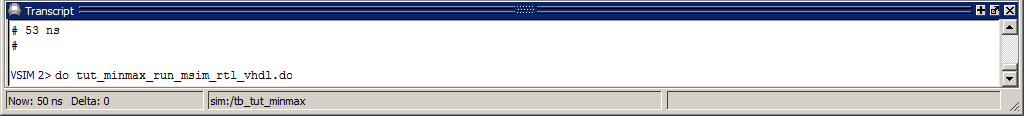
\includegraphics[scale=\tutpicscale]{078rundofileagainfrommodelsim.png}
\caption{Opnieuw uitvoeren van het commando-script.}
\label{fig:078rundofileagainfrommodelsim}
\end{figure}

\section{Pinnen toekennen}
\label{sec:pinnentoekennen}
Voordat we aan de implementatie gaan beginnen, moeten we eerst de fysieke pinnen koppelen 
aan de in- en uitgangen van de VHDL-beschrijving. Dit gebeurt met het onderdeel \textsl{Pin Planner}. 
Helaas weet de Pin Planner nog niet welke in- en uitgangen het ontwerp heeft. Pas na synthese 
zijn deze bekend. Gelukkig hebben we dit al eerder gedaan. Zie de figuren~\ref{fig:080startanalysisandsynthesis} tot en met
\ref{fig:075notsuccessfull}.

Start nu de Pin Planner via de menuoptie \menu{Assignments\pijl{}Pin Planner} in de Project 
Manager (zie figuur~\ref{fig:082startpinplanner}) of gebruik de sneltoetscombinatie \menu{Ctrl+Shift+N}.

\begin{figure}[H]
\centering
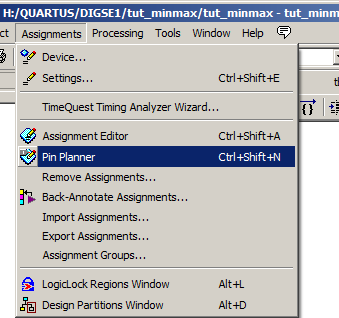
\includegraphics[scale=\tutpicscale]{082startpinplanner.png}
\caption{Starten van de Pin Planner}
\label{fig:082startpinplanner}
\end{figure}
 
In de Pin Planner kunnen de fysieke pinnen aan de in- en uitgangen van de VHDL-beschrijving 
gekoppeld worden. De fysieke pinnen zijn zelf weer verbonden met schakelaars en leds. In de 
twee onderstaande tabellen zijn de koppelingen weergegeven
(tabellen~\ref{tab:inputsdesign} en \ref{tab:outputsdesign}).

\begin{table}[H]
\centering
\caption{Koppelingen ingangen aan pinnen en schakelaars}
\label{tab:inputsdesign}
\begin{tabular}{|p{3cm}|p{3cm}|p{3cm}|}
\hline 
\rb{\textbf{Ingang}} & \rb{\textbf{Pinnaam}} & \rb{\textbf{Schakelaar}} \\ \hline 
\rb{\texttt{a[3]}}   & \rb{\texttt{D2}}      & \rb{\texttt{SW9}} \\ \hline 
\rb{\texttt{a[2]}}   & \rb{\texttt{E4}}      & \rb{\texttt{SW8}} \\ \hline 
\rb{\texttt{a[1]}}   & \rb{\texttt{E3}}      & \rb{\texttt{SW7}} \\ \hline 
\rb{\texttt{a[0]}}   & \rb{\texttt{H7}}      & \rb{\texttt{SW6}} \\ \hline 
\rb{\texttt{b[3]}}   & \rb{\texttt{G4}}      & \rb{\texttt{SW3}} \\ \hline 
\rb{\texttt{b[2]}}   & \rb{\texttt{H6}}      & \rb{\texttt{SW2}} \\ \hline 
\rb{\texttt{b[1]}}   & \rb{\texttt{H5}}      & \rb{\texttt{SW1}} \\ \hline 
\rb{\texttt{b[0]}}   & \rb{\texttt{J6}}      & \rb{\texttt{SW0}} \\ \hline 
\rb{\texttt{minmax}} & \rb{\texttt{J7}}      & \rb{\texttt{SW5}} \\ \hline 
\end{tabular} 
\end{table}

\begin{table}[H]
\centering
\caption{Koppelingen uitgangen aan pinnen en schakelaars}
\label{tab:outputsdesign}
\begin{tabular}{|p{3cm}|p{3cm}|p{3cm}|}
\hline
\rb{\textbf{Uitgang}} & \rb{\textbf{Pinnaam}} & \rb{\textbf{Schakelaar}} \\ \hline 
\rb{\texttt{f[3]}}    & \rb{\texttt{H1}}      & \rb{\texttt{LEDG3}} \\ \hline 
\rb{\texttt{f[2]}}    & \rb{\texttt{J3}}      & \rb{\texttt{LEDG2}} \\ \hline 
\rb{\texttt{f[1]}}    & \rb{\texttt{J2}}      & \rb{\texttt{LEDG1}} \\ \hline 
\rb{\texttt{f[0]}}    & \rb{\texttt{J1}}      & \rb{\texttt{LEDG0}} \\ \hline 
\end{tabular} 
\end{table}

Vul de pinnamen in volgens de tabellen~\ref{tab:inputsdesign} en \ref{tab:outputsdesign}.
Zie figuur~\ref{fig:083pinplannerwithpinsassigned}.

Opmerking: je hoeft alleen het laatste deel van een naam in te voeren, dus D2, E4 etc. Quartus 
zal het woord \naam{PIN\_} voor de pinnaam zetten, dus J2 wordt dan \naam{PIN\_J2}.

Noot: in bijlage~\ref{chap:pinbenaming} is een complete lijst opgenomen met daarin de koppelingen tussen de fysieke 
pinnen en de schakelaars, drukknoppen, leds en 7-segments displays.

\begin{figure}[H]
\centering
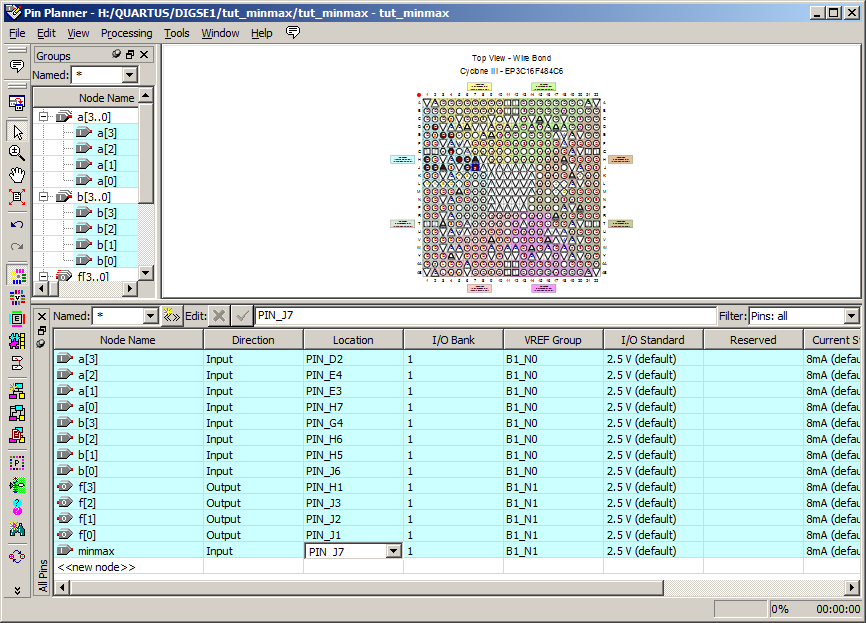
\includegraphics[scale=\tutpicscale]{083pinplannerwithpinsassigned.png}
\caption{Overzicht van de Pin Planner IDE met pinbenaming ingevuld.}
\label{fig:083pinplannerwithpinsassigned}
\end{figure}

Sluit de Pin Planner af via \menu{File\pijl{}Close}. Je hoeft de invoer niet op te slaan, dat gebeurt 
automatisch (er is trouwens geen \naam{save as}-optie). Zie figuur~\ref{fig:084closepinplanner}.
 
\begin{figure}[H]
\centering
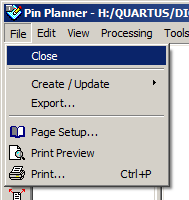
\includegraphics[scale=\tutpicscale]{084closepinplanner.png}
\caption{Afsluiten Pin Planner.}
\label{fig:084closepinplanner}
\end{figure}

Van alle pinnen worden er maar een paar gebruikt. De ongebruikte pinnen worden standaard in 
tri-state met pull-up gezet. Dat is een veilige toestand maar sommige leds gaan dan zwak 
branden. Dat kan tot verwarring leiden. De standaard toestand van de pinnen moet veranderd 
worden in tri-state.

Selecteer in de Program Manager \menu{Assignments\pijl{}Device}. Zie figuur~\ref{fig:085assignmentsdevice}.
 
\begin{figure}[H]
\centering
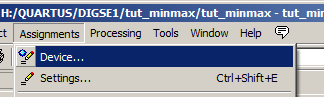
\includegraphics[scale=\tutpicscale]{085assignmentsdevice.png}
\caption{Starten van de Device Settings.}
\label{fig:085assignmentsdevice}
\end{figure}

Er wordt een dialoog geopend (zie figuur~\ref{fig:086deviceoverview}).
Selecteer daar de knop \menu{Device and Pin Options}.

\begin{figure}[H]
\centering
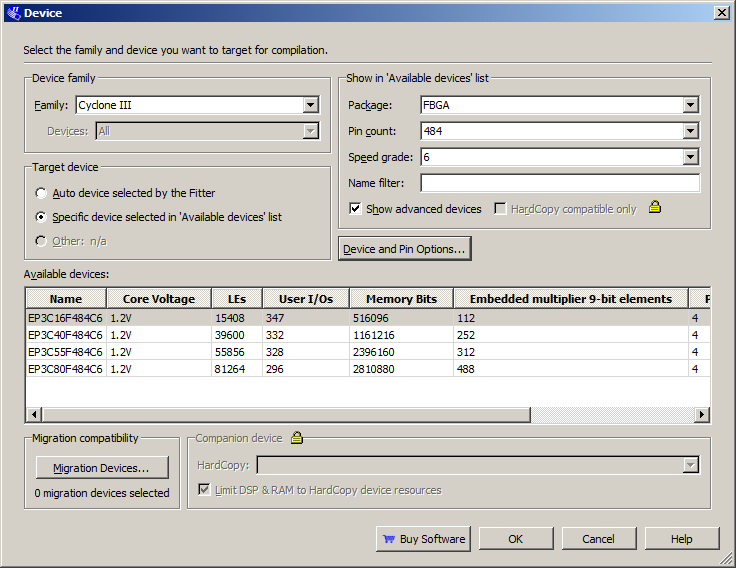
\includegraphics[scale=\tutpicscale]{086Zdeviceoverview.png}
\caption{Overzicht IDE van de Device Settings.}
\label{fig:086deviceoverview}
\end{figure}
 
Er wordt een nieuw dialoog geopend, zie figuur~\ref{fig:087selecttristate}.
Selecteer onder \naam{Catagory:} de optie 
\naam{Unused Pins}. Aan de rechterkant in nu een dropdown-box zichtbaar
met de naam \naam{Reserve all unused pins}.
Selecteer de optie \naam{As input tri-stated}. Klik op \menu{OK}. De dialoog wordt afgesloten en je 
komt weer terug bij het eerste dialoog. Sluit deze af door op \menu{OK} te klikken.

\begin{figure}[H]
\centering
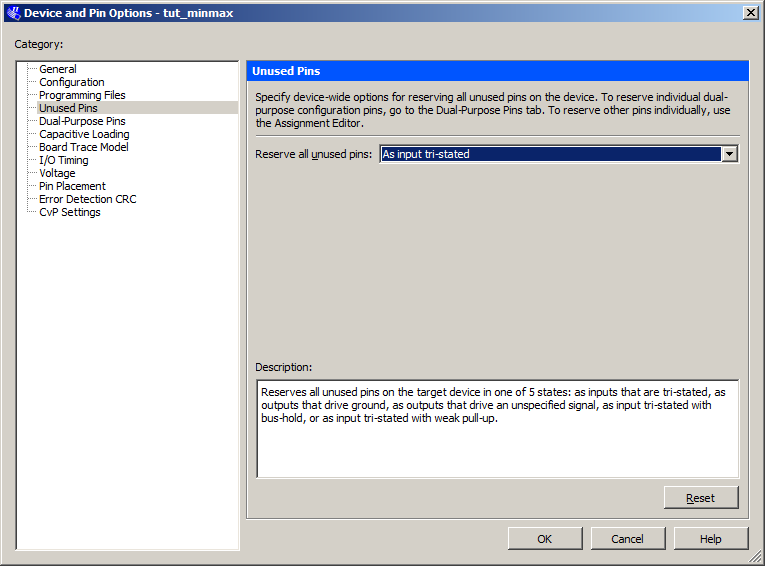
\includegraphics[scale=\tutpicscale]{087selecttristate.png}
\caption{Selecteren van de opties voor de niet-gebruikte pinnen.}
\label{fig:087selecttristate}
\end{figure}

%We gaan nu verder met de compilatie.

\section{Compilatie}
\label{sec:compilatie}
Nu de pinaansluitingen ingevoerd zijn, wordt de VHDL-beschrijving gecompileerd. Compileren 
valt uiteen in twee delen: synthese en implementatie. Synthese houdt in dat de VHDL-code wordt 
vertaald met als resultaat een netlist; een beschrijving van de digitale logica in primitieven. Denk 
hierbij aan poorten, flipflops, LUTs (LookUp Table, ROM) of speciale voorzieningen zoals 
Phase Locked Loops of klokbuffers. Deze primitieven zijn voor elk configureerbaar type weer 
anders. Bij het aanmaken van een nieuw project hebben we al opgegeven welke component we 
gaan gebruiken. Implementatie houdt in dat de primitieven worden \textsl{gemapped} op de LE's. In 
deze fase wordt ook rekening gehouden met pinaansluitingen en timing.

Start de compilatie via de menuoptie \menu{Processing\pijl{}Start Compilation} of gebruik de 
sneltoetscombinatie \menu{Ctrl+L}. Zie figuur~\ref{fig:090startcompilation}.
 
\begin{figure}[H]
\centering
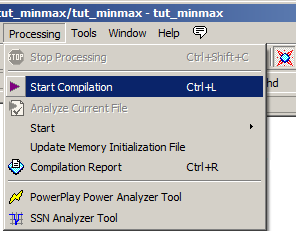
\includegraphics[scale=\tutpicscale]{090startcompilation.png}
\caption{Starten van de compilatie.}
\label{fig:090startcompilation}
\end{figure}

De compilatie wordt nu gestart. Dat kan afhankelijk van het ontwerp enige tijd duren. Je kan de 
voortgang in het \menu{Tasks}-venster. Als de compilatie geen fouten oplevert krijg je een melding 
zoals in figuur~\ref{fig:091compilationsucces}. In het algemeen zijn de waarschuwingen niet problematisch, maar kijk de 
meldigen toch even na.
 
\begin{figure}[H]
\centering
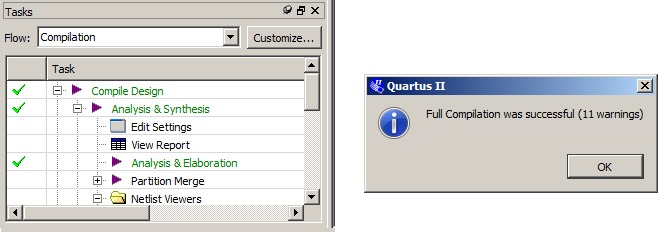
\includegraphics[scale=\tutpicscale]{091compilationsucces.png}
\caption{De compilatie is gelukt.}
\label{fig:091compilationsucces}
\end{figure}

Je krijgt na compilatie een rapport met alle verrichte werkzaamheden. Een interessant onderdeel 
hiervan is het aantal gebruikte LE's. Hieraan kan je zien hoe groot je ontwerp is.
Zie figuur~\ref{fig:092flowsummary}.

\begin{figure}[H]
\centering
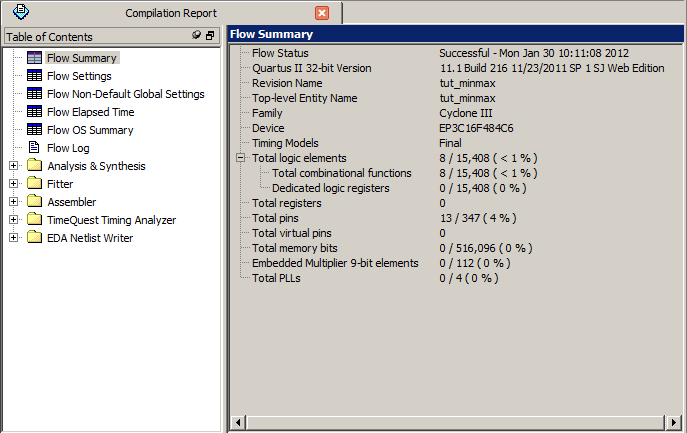
\includegraphics[scale=\tutpicscale]{092flowsummary.png}
\caption{Overzicht van het resultaat van de compilatie.}
\label{fig:092flowsummary}
\end{figure}

De programmatuur is ontwikkeld door Quartus. Er zijn ook andere \textsl{tool chains} verkrijgbaar die 
VHDL-code met hoog abstractieniveau kunnen compileren. Die van Quartus kan dat niet; alleen 
RTL-beschrijvingen (Register Transfer Level) zijn mogelijk. We zullen ons hier aan houden.

\section{Configureren van de Cyclone III}
\label{sec:configureren}

De compilatiestap is nu afgerond: we kunnen verder gaan met het configureren van de Cyclone 
III. We gaan dus het configuratiebestand in deze component laden. Dat gaat volgens het JTAG-
protocol. Dit protocol stelt de gebruiker in staat een hele keten van componenten te configureren. 
Dit is erg handig omdat je zo updates in de componenten kan laden, ook al zijn ze al op een print 
gemonteerd.

%\newpage
Zorg ervoor dat de USB-kabel juist is aangesloten en het ontwikkelbord is aangezet. Als je dit 
vergeet, zal de software een foutmelding geven.

\fpf{Raadpleeg de docent voordat je de apparatuur aansluit en aanzet!}

Selecteer in de Project Manager de menuoptie \menu{Tools\pijl{}Programmer} (figuur~\ref{fig:095startprogrammer}).

\begin{figure}[H]
\centering
\includegraphics[scale=\tutpicscale]{095startprogrammer.png}
\caption{Starten van de programmer.}
\label{fig:095startprogrammer}
\end{figure}

De programmer wordt gestart (figuur~\ref{fig:097programmerwithfileloaded}).

\begin{figure}[H]
\centering
%\includegraphics[scale=\tutpicscale]{097programmerwithfileloaded.png}
\begin{overpic}[scale=\tutpicscale,unit=1mm]{097programmerwithfileloaded.png}
\linethickness{1pt}
\color{red}\put(30,66.2){\oval(35,5)}
\end{overpic}
\caption{Overzicht van de Programmer IDE.}
\label{fig:097programmerwithfileloaded}
\end{figure}

Je kan zien of de programmer het ontwikkelbord 
heeft gevonden als in het veld naast \naam{Hardware Setup} de regel \naam{USB-Blaster [USB-0]} 
staat. Zo niet, klik dan op \menu{Hardware Setup} en selecteer de Blaster. Je ziet ook dat de 
programmer een bestand \naam{tut\_minmax.sof} heeft geselecteerd. Dit is het configuratiebestand 
dat in de Cyclone III geladen moet worden.

Als in het veld naast \naam{Hardware Setup} de opmerking \naam{No Hardware}
staat, klik dan op de knop \menu{Hardware Setup}.
\textbf{\underline{Dubbelklik}} in het geopende dialoogvenster op
\naam{USB-Blaster} in de lijst bij \naam{Available Hardware Items} en klik
daarna op de knop \menu{Close}. Zie figuur~\ref{fig:096addhardware}.
 
\begin{figure}[H]
\centering
\includegraphics[scale=\tutpicscale]{096addhardware.png}
\caption{Selecteren van de USB-Blaster download-hardware.}
\label{fig:096addhardware}
\end{figure}

Druk op Start om de Cyclone III te configureren. Daarna kan je je ontwerp testen door middel 
van de schakelaars.

\section{Gegenereerde hardware}
\label{sec:gegenereerdehardware}

Het is natuurlijk interessant om te bekijken wat de synthese nu eigenlijk voor hardware heeft 
opgeleverd. Dit kan je zien met behulp van de RTL viewer. Dubbelklik in het \naam{Tasks}-venster op 
de regel \menu{RTL Viewer}. Zie figuur~\ref{fig:100startrtlviewer}.

\begin{figure}[H]
\centering
\includegraphics[scale=\tutpicscale]{100startrtlviewer.png}
\caption{Selecteren van de RTL Viewer.}
\label{fig:100startrtlviewer}
\end{figure}

Er wordt een nieuw programma gestart met daar de gegenereerde hardware (figuur~\ref{fig:101rtlviewer}). Let 
wel: dit is nog niet de werkelijke implementatie, alleen primitieven.
 
\begin{figure}[H]
\centering
\includegraphics[scale=\tutpicscale]{101rtlviewer.png}
\caption{Overzicht van de gegenereerde hardware in primitieven.}
\label{fig:101rtlviewer}
\end{figure}

De tutorial is nu ten einde. Veel succes met het practicum.


\ifbetaversion

\chapter{Tips, tricks \& troubleshoot}
In dit hoofdstuk wordt een aantal veel voorkomende problemen toegelicht en hoe
je ze kunt verhelpen. Daarnaast natuurlijk de tips \& tricks.


\section{Foutmelding ``Top-level ... undefined''}
\label{sec:fouttoplevel}
Onderstaande foutmelding geeft aan (zie figuur~\ref{fig:220undefinedtoplevelentity})
dat de ingestelde \textsl{top-level design entity} niet gedefinieerd is. De
kwalificatie \textsl{top-level} slaat op de allerhoogste design entity (denk aan
VHDL-entity) en die kan niet gevonden worden of is niet gedefinieerd.

\begin{figure}[H]
\centering
\includegraphics[scale=\tutpicscale]{220undefinedtoplevelentity.png}
\caption{De top-level entity is niet gevonden.}
\label{fig:220undefinedtoplevelentity}
\end{figure}

Dit gebeurt meestal bij het aanmaken van een nieuw project omdat de verkeerde
naam is ingevuld (zie figuur~\ref{fig:025enterdirandname}). In het voorbeeld is
de naam \naam{opdracht9} ingevuld terwijl bij de \naam{entity}-beschrijving in
VHDL een andere naam is gebruikt. Gelukkig kan in Quartus een andere entity
als top-level worden ingesteld. Selecteer via het menu
\menu{Assignments\pijl{}Settings} of gebruik de sneltoets \menu{Ctrl+Shift+E}
(zie ook figuur~\ref{fig:074assignmentssettings}). Klik in het nieuw geopende dialoog
links boven op \naam{General}.

Rechts kan een ander top-level gekozen worden op op de knop met de drie puntjes
te klikken achter het veld met \naam{Top level entity:} waarna in een klein venster
de nieuwe naam gekozen kan worden. Klik dan op \knop{Ok}. Het kleine venster wordt
afgesloten. Klik in de dialoog eerst op knop \knop{Apply} en daarna op knop \knop{Ok}.
De dialoog wordt afgesloten. Zie figuur~\ref{fig:222selecttoplevelentity}.

In de Program Navigator is nu de nieuwe top-level entity te vinden.

\begin{figure}[H]
\centering
\includegraphics[scale=\tutpicscale]{222selecttoplevelentity.png}
\caption{Selectie van top-level entity.}
\label{fig:222selecttoplevelentity}
\end{figure}


\section{Instellen pad naar ModelSim}
\label{chap:instellenmodelsimpad}
Als in Quartus het pad naar ModelSim niet correct is ingesteld, krijg je de volgende foutmelding 
(figuur~\ref{fig:210modelsimpath_121}).

\begin{figure}[H]
\centering
\includegraphics[scale=\tutpicscale]{210modelsimpath_121.png}
\caption{De simulator kan niet worden gestart.}
\label{fig:210modelsimpath_121}
\end{figure}

Ga als volgt te werk:

\begin{itemize}\itemsep-1pt
\item Open in de Project manager het menu \menu{Tools\pijl{}Options}
\item In het venster dat geopend wordt kies je \menu{EDA Tool Options}
\item Aan de rechterkant kan je in het veld \naam{ModelSim-Altera} het pad opgeven.
\item Voor de PC's op school is dat \lstinline|C:\altera\13.0sp1\modelsim_ase\win32aloem|
\end{itemize}

Op je eigen PC of laptop hangt dat af van het installatie-pad. Zie
figuur~\ref{fig:212modelsimpath2}.

Tip: bij gebruik van Quartus v13.1 moet je een \lstinline|\| (''backslash'')
achter de padnaam zetten.

\begin{figure}[H]
\centering
\includegraphics[scale=\tutpicscale]{212modelsimpath2.png}
\caption{Instellen van pad naar ModelSim.}
\label{fig:212modelsimpath2}
\end{figure}


\section{Smart compilation}
Quartus heeft de neiging om bij een compilatie-opdracht alle stappen te
doorlopen, ook als dat niet nodig is. Denk bijvoorbeeld aan het instellen van
een nieuwe top-level entity. Dan is synthese niet nodig, die is al een keer
uitgevoerd. Als een project meerdere VHDL-bestanden bevat, is het niet nodig
om alle bestanden opnieuw te synthetiseren, alleen de bestanden die aangepast
zijn.

Quartus heeft een optie die \textsl{Smart compilation} wordt genoemd en
alleen die stappen doorloopt die nodig zijn voor het eindresultaat. Open via
het menu \menu{Assignments\pijl{}Settings}. Selecteer in het gedeelte
\naam{Catagory} de optie \naam{Compilation Process Settings}. Aan de 
rechterkant verschijnen de instellingen voor compilatie. Zet een vinkje
bij de optie \naam{Use smart compilation} en sluit het venster af
door eerst op knop \knop{Apply} te drukken en daarna op knop \knop{Ok}.
Zie figuur~\ref{fig:225smartcompilation}.

\begin{figure}[H]
\centering
\includegraphics[scale=\tutpicscale]{225smartcompilation.png}
\caption{Instellen van van de optie Smart compilation.}
\label{fig:225smartcompilation}
\end{figure}

\section{Quartus blijft hangen}
Er is een aantal situaties waardoor Quartus blijft hangen en alleen maar
via de Task Manager van Windows kan worden afgesloten. Hieronder de lijst met
bekende problemen:

\begin{itemize}\itemsep-1pt
\item Bij het aanmaken van een nieuw project is als projectmap een map gekozen
      waar je als gebruiker geen schrijfrechten voor hebt. Een mooi voorbeeld
      is de map \lstinline|C:\altera\11.1|, de installatiemap van Quartus.
      Deze map wordt standaard opgegeven bij het aanmaken van een nieuw
      project. De oplossing is uiteraard eenvoudig: selecteer een andere map.
\item De bestanden van het project staan opgeslagen op de H:-schijf. Soms is
      deze schijf tijdelijk niet beschikbaar, bijvoorbeeld als gevolg door
      veel gebruikers. De oplossing: gewoon even wachten, na een tijdje
      reageert Quartus weer.
\end{itemize}

\fi


\section{Ingestelde pad naar ModelSim wordt niet opgeslagen}
Het is een paar keer gebleken dat, ondanks dat het pad naar de ModelSim
executable ingesteld is, ModelSim niet gestart kan worden. Dit komt vooral
voor bij versie 13.1 van Quartus. Het is mogelijk om handmatig een
verwijzing in te stellen naar de ModelSim executable.

\begin{itemize}\itemsep-1pt
\item Open de map waar het gebruikerprofiel is opgeslagen, meestal iets in
      de trant van \lstinline|C:\Users\<gebruikersnaam>|
\item Open het initialisatie-bestand \lstinline|quartus2.ini|
\item Voeg de volgende code toe, uiteraard met de juiste padnaam
\begin{lstlisting}[language=VHDL,numbers=none,belowskip=-3.5ex]
[EDA_Tool_Paths 13.1]
EDA_TOOL_PATH_MODELSIM_ALTERA = C:\altera\13.1\modelsim_ae\win32aloem
\end{lstlisting}
\item Sluit het bestand
\item Start Quartus opnieuw op

\end{itemize}

\section{Gebruik USB-Blaster onder Linux}
Als je onder Linux als gewone gebruiker inlogt, kan je niet direct gebruik
maken van de USB-aansluiting. Je krijgt dan een foutmelding zoals te zien is
in figuur \ref{fig:230jtagerror89}.

%\begin{itemize}\itemsep-1pt
%\item[] \lstinline|Unexpected error code 0x89, operation failed.|
%\end{itemize}

\begin{figure}[H]
\centering
\includegraphics[scale=\tutpicscale]{231Aquartus_errorCode_89}
\caption{Foutmelding bij programmeren onder Linux.}
\label{fig:230jtagerror89}
\end{figure}

Voer de volgende handelingen uit om als gewone gebruiker de USB-Blaster te
kunnen gebruiken. De handelingen zijn getest op CentOS 6.5. De handelingen
moet je als gebruiker \lstinline|root| uitvoeren.

\begin{itemize}\itemsep-1pt
\item Maak een bestand \lstinline|40-usbblaster.rules| aan in de map
      \lstinline|/etc/udev/rules.d|
\item Plaats in het bestand de volgende code:
\begin{lstlisting}[language=VHDL,numbers=none,belowskip=-3.5ex]
# USB-Blaster

SUBSYSTEM=="usb", ENV{DEVTYPE}=="usb_device", ATTRS{idVendor}=="09fb", ATTRS{idProduct}=="6001", MODE="0666", SYMLINK+="usbblaster/%k"
SUBSYSTEM=="usb", ENV{DEVTYPE}=="usb_device", ATTRS{idVendor}=="09fb", ATTRS{idProduct}=="6002", MODE="0666", SYMLINK+="usbblaster/%k"
SUBSYSTEM=="usb", ENV{DEVTYPE}=="usb_device", ATTRS{idVendor}=="09fb", ATTRS{idProduct}=="6003", MODE="0666", SYMLINK+="usbblaster/%k"

# USB-Blaster II
SUBSYSTEM=="usb", ENV{DEVTYPE}=="usb_device", ATTRS{idVendor}=="09fb", ATTRS{idProduct}=="6010", MODE="0666", SYMLINK+="usbblaster2/%k"
SUBSYSTEM=="usb", ENV{DEVTYPE}=="usb_device", ATTRS{idVendor}=="09fb", ATTRS{idProduct}=="6810", MODE="0666", SYMLINK+="usbblaster2/%k"
\end{lstlisting}
\item Sluit het bestand
\item Herlees de udev-regels met \lstinline|udevadm control --reload-rules|
\item Trigger de updates met \lstinline|udevadm trigger|
\item Herstart de progammer-software
\end{itemize}


\section{Design Rule S102}
Als je de melding \lstinline|S102: Synchronous Port and Asynchronous Port of the Same Register Should Not Be Driven by the Same Signal Source|
krijgt, heb je waarschijnlijk een asynchrone \'{e}n synchrone reset in je
ontwerp gebruikt. Zoek alle deelontwerpen af naar deze twee vormen en verander
alle synchrone resets in asynchrone resets. Zie
\url{http://quartushelp.altera.com/13.0/mergedProjects/verify/da/comp_file_rules_synch_reset.htm}
en klik op de \textsl{buttons} om de schema's te openen.

\section{Naamgeving bestanden en entity's}
Een \textsl{entity} is een hardware-eenheid en levert bij synthese
dus hardware op. Een \textsl{bestandsnaam} is de naam van het bestand
waarin de hardware beschreven of getekend is. De entity-naam is
onafhankelijk van het gebruikte besturingssysteem, de bestandsnaam is
wel afhankelijk.

In Quartus zijn schemabestanden met de extensie \naam{.bdf}
gekoppeld aan de entity-naam: de bestandsnaam zonder de extensie
is gelijk ook de entity-naam.

Bij beschrijvingstalen als VHDL en Verilog ligt dat anders: de
bestandsnaam hoeft niet hetzelfde te zijn als de entity-naam. In feite
is het bestand een \textsl{container} met daarin de beschrijving
van de hardware. ModelSim gebruikt de bestandsnaam om de beschrijving
te compileren (bv.\@ met \naam{vcom} en \naam{vlog}) maar gebruikt de
entity-naam bij het starten van de simulatie (m.b.v.\@ \naam{vsim}).

Let op: entity-namen mogen \textsl{niet} beginnen met een cijfer of
een leesteken. In feite gelden voor de entity-namen dezelfde regels als
voor variabelen. Schemabestandsnamen mogen dus ook niet met een cijfer
of een leesteken beginnen, VHDL-bestandsnamen wel.

Het is verstandig om de bestandsnaam en de entity-naam hetzelfde te houden.
Dat voorkomt allerlei problemen. Plaats maximaal \'e\'en design
(entity en architecture) in \'e\'en bestand.

Gebruik voor testbenches dezelfde naamgeving als de entity die gesimuleerd
moeten worden met \lstinline|tb_| ervoor. Doe dat ook voor de entitynaam van
de testbench. Modelsim command scripts eindigen op de extensie \lstinline|.do|
en starten over het algemeen de simulator met als top level de testbench.
Zie onderstaand stukje code.

\begin{lstlisting}[language=tclfix,numbers=none,belowskip=-3.5ex]
# This file is named 'tb_entityname.do'
...
vcom entityname.vhd      # file containing design entity 'entityname'
vcom tb_entityname.vhd   # file containing testbench entity 'tb_entityname'
vsim tb_entityname       # Simulator top level is 'tb_entityname'
...
\end{lstlisting}

\section{Pinnen worden niet getoond in de Pin Planner}
Als de pinnen niet worden getoond in de Pin Planner, heb je waarschijnlijk
geen \textsl{Device Type} opgegeven en staat het type op \textsl{Auto}. Ga
via menu \menu{Assignments\pijl{}Device} en vul de juiste gegevens in.
Zie ook figuur~\ref{fig:028familydevicesettings}.

\section{Verkeerde pinnen worden getoond}
Dan heb je de verkeerde entity als top-level ingesteld. Zie
paragraaf~\ref{sec:fouttoplevel}.

\section{ModelSim stopt na enige tijd}
Als ModelSim na enige tijd stopt voordat de simulatie werkelijk gestart
wordt, dan ben je vergeten om de do-file op te geven (in Quartus). Zie de
figuren \ref{fig:074assignmentssettings} en \ref{fig:073settingssimulation}.

\section{``Instance ... is not bound''}
Deze foutmelding wordt gegenereerd door ModelSim. Het betekent dat binnen de
simulatie-omgeving geen entity met die naam is gedefinieerd en er kan dus geen
instantie van worden aangemaakt. De simulatie gaat wel verder. Dat levert
uiteraard problemen op. De werking is van het te simuleren systeem is niet
correct, want er mist een deel. Interne signalen van de
niet-ge\"instanti\"eerde entity zijn niet beschikbaar. Mogelijke oorzaken zijn:
\begin{itemize}
\item Het VHDL-bestand met de betreffende entity wordt niet gecompileerd
      (de \texttt{vcom}-opdracht is niet correct of vergeten).      
\item Bij instanti\"ering wordt een entity-naam opgegeven die in geen van
      de  gecompileerde VHDL-bestanden is opgegeven.
\end{itemize}

\section{Opruimen van een Quartus-project}
Quartus heeft de neiging om tijdens compilatie ontzettend veel, vooral kleine
bestanden aan te maken. Je kan heel veel van die bestanden en mappen gewoon
verwijderen als je project is afgerond.

%%%De mappen \lstinline|db|, \lstinline|incremental_db|, \lstinline|output_files|
%%%en \lstinline|simulation| kan je gewoon verwijderen. Let erop dat je geen
%%%eigen aangemaakte bestanden in de map \lstinline|simulation| moet hebben staan.

Onderstaand script kan je draaien in een Windows-command box en verwijdert
bijna elk bestand dat niet nodig is inclusief een aantal mappen die door
Quartus en ModelSim aangemaakt worden.

\lstinputlisting[label=cod:opruim,caption=Windows opruimscript,numbers=none]{remove_unwanted_files.cmd}


\appendix

%\chapter{Knoppen en sneltoetscombinaties}
\chapter{Knoppen en sneltoetsen}
\label{chap:knoppenensneltoetscombinatie}
In deze bijlage is een tabel opgenomen met een aantal knoppen en sneltoetscombinaties. Niet alle 
knoppen worden in deze tutorial gebruikt.

%\newcolumntype{V}{>{\centering\arraybackslash} m{3cm} }

\begin{table}[H]
%\renewcommand\arraystretch{1.0}
\caption{Knoppen en sneltoetscombinaties.}
\label{tab:knoppenensneltoetscombinaties}
\centering
\begin{tabular}[t]{|c|p{4.9cm}|p{6.5cm}|l|}
\hline
& & & \\[-2ex]
\textbf{Knop} & \textbf{Benaming} & \textbf{Menu} & \textbf{Sneltoets} \\ [0.7ex] \hline
\parbox[c][2.5em]{2em}{\includegraphics[scale=1]{112viewprojectnavigator}} & View Project Navigator & \vspace*{-17pt}\naam{View\pijl{}Utility Windows\pijl{}Project Navigator} & Alt+0 \\ \hline
\parbox[c][2.5em]{2em}{\includegraphics[scale=1]{111device}} & Device Assignments & \naam{Assignments\pijl{}Device} & - \\ \hline
\parbox[c][2.5em]{2em}{\includegraphics[scale=1]{113settings}} & Settings Assignments & \naam{Assignments\pijl{}Settings} & Ctrl+Shift+E \\ \hline
\parbox[c][2.5em]{2em}{\includegraphics[scale=1]{114assignmenteditor}} & Assignment Editor* & \naam{Assignments\pijl{}Editor} & Ctrl+Shift+A \\ \hline
\parbox[c][2.5em]{2em}{\includegraphics[scale=1]{115pinplanner}} & Pin Planner & \naam{Assignments\pijl{}Pin Planner} & Ctrl+Shift+N \\ \hline
\parbox[c][2.5em]{2em}{\includegraphics[scale=1]{116floorplanner}} & Floor Planner* & \naam{Tools\pijl{}Chip Planner} & - \\ \hline
\parbox[c][2.5em]{2em}{\includegraphics[scale=1]{117startcompilation}} & Start Compilation & \naam{Processing\pijl{}Start Compilation} & Crtl+L \\ \hline
\parbox[c][2.5em]{2em}{\includegraphics[scale=1]{118startanalysisandsynthesis}} & Start Analysis & \vspace*{-17pt}\naam{Processing\pijl{}Start\pijl{}Start Analysis \& Synthesis} & Crtl+K \\ \hline
\parbox[c][2.5em]{2em}{\includegraphics[scale=1]{119startiminganalyser}} & \vspace*{-17pt}Start TimeQuest Timing Analyser* & \vspace*{-17pt}\naam{Processing\pijl{}Start\pijl{} Start TimeQuest Timing Analyser} & Ctrl+Shift+T \\ \hline
\parbox[c][2.5em]{2em}{\includegraphics[scale=1]{120timinganalyser}} & \vspace*{-17pt}Open TimeQuest Timing Analyser* & \vspace*{-17pt}\naam{Tools\pijl{}TimeQuest Timing Analyser} & - \\ \hline
\parbox[c][2.5em]{2em}{\includegraphics[scale=1]{121rtlsimulation}} & RTL Simulation & \vspace*{-17pt}\naam{Tools\pijl{}Run Simulation Tools\pijl{}RTL Simulation} & - \\ \hline
\parbox[c][2.5em]{2em}{\includegraphics[scale=1]{122gatelevelsimulation}} & Gate Level Simulation* & \vspace*{-17pt}\naam{Tools\pijl{}Run Simulation Tools\pijl{}Gate Level Simulation} & - \\ \hline
\parbox[c][2.5em]{2em}{\includegraphics[scale=1]{123compilationreport}} & Compilation Report & \naam{Processing\pijl{}Compilation Report} & Crtl+R \\ \hline
\parbox[c][2.5em]{2em}{\includegraphics[scale=1]{124programmer}} & Programmer & \naam{Tools\pijl{}Programmer} & - \\ \hline
\parbox[c][2.5em]{2em}{\includegraphics[scale=1]{125analysecurrentfile}} & Analyse Current File & \vspace*{-17pt}\naam{Processing\pijl{}Analyse Current File} & - \\ \hline
\parbox[c][2.5em]{2em}{\includegraphics[scale=1]{126inserttemplate}} & Insert Template & \naam{Edit\pijl{}Insert Template} & - \\ \hline
\end{tabular}
\end{table}
\vskip-4ex
* Wordt niet gebruikt tijdens deze tutorial.


\chapter{Pinbenaming EP3C16F484C-6N}
\label{chap:pinbenaming}
In deze bijlage vind je de pinbenaming terug. Er staan ook opmerkingen bij.

\begin{table}[H]
\centering
\caption{Pinbenamingen FPGA, deel 1.}
\label{tab:pinbenamingenfpga1}
\begin{tabular}[t]{|p{3cm}|p{3cm}|p{2cm}|p{5cm}|}
\hline 
\rb{Type}         & \rb{Naam}  & \rb{Pinnaam} & \rb{Opmerking} \\ \hline 
                  &                &          &   \\  \hline 
\rb{Clock}        & \rb{CLOCK\_50} & \rb{G21} & \rb{Global Clock 1} \\  \hline 
                  &                &          &   \\  \hline 
\rb{Push Buttons} & \rb{BUTTON[0]} & \rb{H2}  & \rb{Ontdenderd, actief laag} \\  \hline 
                  & \rb{BUTTON[1]} & \rb{G3}  &   \\  \hline 
                  & \rb{BUTTON[2]} & \rb{F1}  &   \\  \hline 
                  &                &          &   \\  \hline 
\rb{Switches}     & \rb{SW[0]}     & \rb{J6}  & \rb{Niet ontdenderd, actief hoog} \\  \hline
                  & \rb{SW[1]}     & \rb{H5}  &  \\  \hline
                  & \rb{SW[2]}     & \rb{H6}  &  \\  \hline
                  & \rb{SW[3]}     & \rb{G4}  &  \\  \hline
                  & \rb{SW[4]}     & \rb{G5}  &  \\  \hline
                  & \rb{SW[5]}     & \rb{J7}  &  \\  \hline
                  & \rb{SW[6]}     & \rb{H7}  &  \\  \hline
                  & \rb{SW[7]}     & \rb{E3}  &  \\  \hline
                  & \rb{SW[8]}     & \rb{E4}  &  \\  \hline
                  & \rb{SW[9]}     & \rb{D2}  &  \\  \hline
                  &                &          &   \\  \hline 
\rb{Leds}         & \rb{LEDG[0]}   & \rb{J1}  & \rb{Actief hoog} \\ \hline
                  & \rb{LEDG[1]}   & \rb{J2}  & \\ \hline
                  & \rb{LEDG[2]}   & \rb{J3}  & \\ \hline
                  & \rb{LEDG[3]}   & \rb{H1}  & \\ \hline
                  & \rb{LEDG[4]}   & \rb{F2}  & \\ \hline
                  & \rb{LEDG[5]}   & \rb{E1}  & \\ \hline
                  & \rb{LEDG[6]}   & \rb{C1}  & \\ \hline
                  & \rb{LEDG[7]}   & \rb{C2}  & \\ \hline
                  & \rb{LEDG[8]}   & \rb{B2}  & \\ \hline
                  & \rb{LEDG[9]}   & \rb{B1}  & \\ \hline
\end{tabular} 
\end{table}
\vspace*{-2ex}
Dit zijn de benamingen zoals ze in de documentatie van het DE0-bordje worden
gebruikt. Je kan ook je eigen namen gebruiken. Quartus zal, wanneer van
toepassing, het woord \naam{PIN\_} voor de pinnaam zetten, dus J2 wordt dan 
\naam{PIN\_J2}.

Op de volgende pagina staan de pingegevens van de 7-segment displays. Tevens
is de layout gegeven.

\newpage
\begin{table}[H]
\centering
\caption{Pinbenamingen FPGA, deel 2.}
\label{tab:pinbenamingenfpga2}
\begin{tabular}{|m{3cm}|m{3cm}|m{2cm}|m{5cm}|}
\hline 
\rb{Type}      & \rb{Naam}  & \rb{Pinnaam}  & \rb{Opmerking} \\ \hline 
               &                 &          &   \\  \hline 
\rb{7-segment} & \rb{HEX0\_D[0]} & \rb{E11} & \rb{Alle actief laag} \\  \hline
               & \rb{HEX0\_D[1]} & \rb{F11} &  \\  \hline
               & \rb{HEX0\_D[2]} & \rb{H12} &  \\  \hline
               & \rb{HEX0\_D[3]} & \rb{H13} &  \\  \hline
               & \rb{HEX0\_D[4]} & \rb{G12} &  \\  \hline
               & \rb{HEX0\_D[5]} & \rb{F12} &  \\  \hline
               & \rb{HEX0\_D[6]} & \rb{F13} &  \\  \hline
               & \rb{HEX0\_DP}   & \rb{D13} &  \\  \hline
               &                 &          &   \\  \hline 
               & \rb{HEX1\_D[0]} & \rb{A13} &  \\  \hline
               & \rb{HEX1\_D[1]} & \rb{B13} &  \\  \hline
               & \rb{HEX1\_D[2]} & \rb{C13} &  \\  \hline
               & \rb{HEX1\_D[3]} & \rb{A14} &  \\  \hline
               & \rb{HEX1\_D[4]} & \rb{B14} &  \\  \hline
               & \rb{HEX1\_D[5]} & \rb{E14} &  \\  \hline
               & \rb{HEX1\_D[6]} & \rb{A15} &  \\  \hline
               & \rb{HEX1\_DP}   & \rb{B15} &  \\  \hline
               &                 &          &   \\  \hline 
               & \rb{HEX2\_D[0]} & \rb{D15} &  \\  \hline
               & \rb{HEX2\_D[1]} & \rb{A16} &  \\  \hline
               & \rb{HEX2\_D[2]} & \rb{B16} &  \\  \hline
               & \rb{HEX2\_D[3]} & \rb{E15} &  \\  \hline
               & \rb{HEX2\_D[4]} & \rb{A17} &  \\  \hline
               & \rb{HEX2\_D[5]} & \rb{B17} &  \\  \hline
               & \rb{HEX2\_D[6]} & \rb{F14} &  \\  \hline
               & \rb{HEX2\_DP}   & \rb{A18} &  \\  \hline
               &                 &          &   \\  \hline 
               & \rb{HEX3\_D[0]} & \rb{B18} &  \\  \hline
               & \rb{HEX3\_D[1]} & \rb{F15} &  \\  \hline
               & \rb{HEX3\_D[2]} & \rb{A19} &  \\  \hline
               & \rb{HEX3\_D[3]} & \rb{B19} &  \\  \hline
               & \rb{HEX3\_D[4]} & \rb{C19} &  \\  \hline
               & \rb{HEX3\_D[5]} & \rb{D19} &  \\  \hline
               & \rb{HEX3\_D[6]} & \rb{G15} &  \\  \hline
               & \rb{HEX3\_DP}   & \rb{G16} &  \\  \hline
\end{tabular} 
\end{table}
\vspace*{-2.0ex}
\begin{figure}[H]
\centering
\includegraphics[scale=0.25]{004layout7seg.png}
\caption{Layout 7-segment displays}
\label{fig:004layout7seg}
\end{figure}

\end{document} 
